\chapter{机制图与结构示意图}

研究生小周在写一篇关于骨骼肌胰岛素抵抗的论文时，想在引言后的第一张图里交代经典的胰岛素促进葡萄糖转运蛋白4（GLUT4）转位通路。她打开图像生成工具，输入了一句英文要求：“画一张专业、美观的胰岛素信号与GLUT4转位机制图，适合顶级期刊发表。”不到一分钟，画面生成完毕：深蓝紫色的三维细胞背景上漂浮着带高光的蛋白质球体，金黄色的磷酸化光斑沿着发光箭头指向细胞膜，角落里还绘出了细胞核、粗面内质网、高尔基体与微管束。小周觉得画面远比自己用图形软件拼出来的精致，便直接放进了初稿。

导师和同门师兄在组会上审阅这张图时，三分钟内指出了四处硬伤：第一，丝氨酸/苏氨酸激酶 Akt 到下游底物 AS160 被画成了实心激活箭头，而生物学事实是 Akt 磷酸化并抑制 AS160 的 GTP 酶激活蛋白（GAP）活性；第二，激活 Akt 所需的哺乳动物雷帕霉素靶蛋白复合物2（mTORC2）支路完全缺失；第三，调节囊泡运输的小 G 蛋白 Rab 悬空漂在细胞质中央，没有结合在储存囊泡表面；第四，配体结合、脂质转化、激酶级联、囊泡移动与跨膜物质转运全部使用同一种白色实心箭头，读者无法区分哪一步是化学修饰、哪一步是空间位移。

审稿人挑剔机制图或结构示意图时，看的不是三维光影、渐变质感或背景装饰，而是图中包含的每一个科学陈述是否成立。机制图画的不是名词清单，而是对象之间的因果与空间关系；结构示意图画的也不是外观效果，而是组件的几何层序、材料配对与过程方向。只要输入指令里没有给出明确的关系表、线型定义与空间分区，生成模型就会用似是而非的连线填补空白。本章围绕细胞信号机制图与电化学器件截面图两个案例，说明如何把确立的科学知识拆解为可核查的关系与层序，驱动 AI 生成干净的无字底图，再通过排版层叠加标签、箭头与图例。

\section{机制图要交代的四件事}

动笔或输入提示词之前，作者需要先明确一张机制图向读者传递哪几类信息。无论是分子生物学中的信号转导通路、催化化学中的反应循环，还是环境科学中的污染物迁移转化路径，合格的机制图都必须交代四件事：对象、位置、相互作用与证据状态（图~\ref{fig:ch07-01}）。

\begin{figure}[htbp]\centering
% FIG ch07-01 mechanism grammar (Chinese labels)
\begin{tikzpicture}[
  font=\sffamily\small,
  paneltitle/.style={font=\sffamily\bfseries\footnotesize, text=BookInk, anchor=west},
  foot/.style={font=\sffamily\scriptsize, text=BookInk!80},
  infobox/.style={
    draw=BookRule, line width=0.6pt, rounded corners=2pt, fill=BookPale,
    font=\sffamily\scriptsize, align=center,
    text width=48mm, minimum height=9mm, inner sep=2.6pt
  },
  band/.style={
    draw=BookRule, line width=0.5pt,
    font=\sffamily\scriptsize, align=left,
    text width=48mm, minimum height=6.4mm, inner sep=2.4pt
  },
  evbox/.style={
    draw=BookRule, line width=0.5pt, fill=BookPale,
    font=\sffamily\scriptsize, align=left,
    text width=48mm, minimum height=13mm, inner sep=2.6pt
  },
]
\definecolor{ch07act}{HTML}{3A3A3A}
\definecolor{ch07conv}{HTML}{7A7A7A}
\definecolor{ch07trans}{HTML}{E39B5B}
\definecolor{ch07flux}{HTML}{C46A2A}
\definecolor{ch07phos}{HTML}{E3B23C}
\definecolor{ch07hyp}{HTML}{9A9A9A}

\node[paneltitle] (tObj) at (0,0) {对象};
\node[infobox, anchor=north west] (bObj) at ([yshift=-1.2mm]tObj.south west) {是什么\\出现几次};

\node[paneltitle, anchor=north west] (tComp) at ([yshift=-3.2mm]bObj.south west) {位置};
\node[band, fill=BookPale!50, anchor=north west] (bExt) at ([yshift=-1.2mm]tComp.south west) {胞外};
\node[band, fill=white, anchor=north west] (bMem) at ([yshift=-1.1mm]bExt.south west) {质膜};
\node[band, fill=BookPale!30, anchor=north west] (bCyt) at ([yshift=-1.1mm]bMem.south west) {胞质};

\node[paneltitle, anchor=north west] (tInt) at ([yshift=-3.2mm]bCyt.south west) {相互作用};
\node[band, fill=BookPale, minimum height=7.2mm, align=center, anchor=north west]
  (bInt) at ([yshift=-1.2mm]tInt.south west)
  {\tikz[baseline=-0.55ex]{\draw[-{Stealth[length=2mm]}, ch07act, line width=0.8pt] (0,0) -- (32mm,0);}};

\node[paneltitle, anchor=north west] (tEv) at ([yshift=-3.2mm]bInt.south west) {证据状态};
\node[evbox, anchor=north west] (bEv) at ([yshift=-1.2mm]tEv.south west) {%
  \begin{tabular}{@{}l@{\hspace{1.8mm}}l@{}}
    \tikz[baseline=-0.55ex]{\draw[ch07act, line width=0.8pt] (0,0) -- (16mm,0);} & 确立 \\[1.4mm]
    \tikz[baseline=-0.55ex]{\draw[ch07hyp, line width=0.8pt, dashed] (0,0) -- (16mm,0);} & 假设
  \end{tabular}};

\node[paneltitle] (rt) at (60mm,0) {线型图例（本章约定）};
\draw[-{Stealth[length=2mm]}, ch07act, line width=0.8pt] (60mm,-8mm) -- (78mm,-8mm);
\node[anchor=west, font=\sffamily\small] at (82mm,-8mm) {激活};
\draw[-{Bar[width=6pt]}, ch07act, line width=0.8pt] (60mm,-15.5mm) -- (78mm,-15.5mm);
\node[anchor=west, font=\sffamily\small] at (82mm,-15.5mm) {抑制};
\draw[ch07conv, line width=0.5pt] (60mm,-23mm) .. controls (66mm,-21.2mm) and (72mm,-24.8mm) .. (76mm,-23mm);
\draw[-{Straight Barb[open]}, ch07conv, line width=0.5pt] (76mm,-23mm) -- (78mm,-23mm);
\node[anchor=west, font=\sffamily\small] at (82mm,-23mm) {酶促转化};
\draw[ch07trans, line width=1.5pt, dashed, -{Stealth[length=2.5mm, open]}] (60mm,-30.5mm) -- (78mm,-30.5mm);
\node[anchor=west, font=\sffamily\small] at (82mm,-30.5mm) {囊泡转位};
\draw[ch07flux, line width=0.8pt, dotted, -{Stealth[length=2mm]}] (60mm,-38mm) -- (78mm,-38mm);
\node[anchor=west, font=\sffamily\small] at (82mm,-38mm) {物质流动};
\draw[ch07hyp, line width=0.8pt, dashed, -{Stealth[length=2mm]}] (60mm,-45.5mm) -- (78mm,-45.5mm);
\node[anchor=west, font=\sffamily\small] at (82mm,-45.5mm) {假设关系};
\fill[ch07phos] (62mm,-53mm) circle (2pt);
\node[anchor=west, font=\sffamily\small] at (82mm,-53mm) {磷酸化（琥珀色圆点）};
\node[anchor=north west, font=\sffamily\scriptsize, text=BookInk!70, align=left, text width=68mm]
  at (60mm,-58mm) {本例 Figure~1 不含假设关系};

\node[foot, anchor=north west] at ([yshift=-3mm]current bounding box.south west)
  {线型含义以本图图例为准；参照学科惯例（如 SBGN）。};
\end{tikzpicture}

\caption{机制图需要交代的四类信息与本章使用的线型约定。每种关系类型只用一种线型；假设关系与确立关系必须可区分。线型含义由图例定义，并参照学科惯例。}\label{fig:ch07-01}
\end{figure}

\textbf{第一件事是对象：它是什么，在图中出现几次。} 机制图中的每个图形元素都代表一个实体，如小分子配体、跨膜受体、胞内激酶、膜脂或储存囊泡。如果同一个分子在图中出现两次，读者自然会问：这代表两个亚基、两种构象，还是两个时刻的位置？缺乏明确规则时，图像模型常为填满画面而复制图标，例如在细胞膜上并排画六个转运体。因此，整理对象清单时不仅要列出名称，还要规定出现次数。凡是代表单一功能节点的分子（如胰岛素受体、IRS-1、PI3K、PDK1、Akt、mTORC2、AS160），在全图中只出现一次；只有当机制本身涉及空间转移——如 GLUT4 先嵌在胞内储存囊泡膜上（储存态），融合后又插入细胞质膜（功能态）——才允许出现两处，且两处的形状与颜色必须一致。

对象造型还要把握“必要的结构细节”。机制图的任务是讲清因果链条，而非替代结构生物学的原子模型。只画那些省略后会影响理解的特征：如胰岛素受体必须跨膜，才能解释它如何把胞外信号传到胞内；Rab 蛋白必须附着在储存囊泡外表面，才能解释它如何调控囊泡移动。至于胰岛素受体 $\alpha_2\beta_2$ 四聚体的二硫键细节，或 PI3K 中 p85 与 p110 亚基的界面，并非背景图要讨论的问题，交给模型绘制反而容易失真，应简化为简洁轮廓并在图注说明。

\textbf{第二件事是位置：空间分区本身就是信息。} 许多初学者把细胞膜、细胞核或相界面当成装饰背景，这是导致定位错误的根源。在胰岛素通路中，胰岛素只能停留在胞外区与受体胞外域接触；磷脂酰肌醇二磷酸（$\text{PIP}_2$）与三磷酸（$\text{PIP}_3$）锚定在质膜内叶，不能画成漂在胞质深处的圆球；PDK1 与 Akt 需通过 PH 结构域结合到质膜内叶的 $\text{PIP}_3$ 上才能完成激活，因此必须紧贴质膜内侧。把画布划分为“胞外—质膜—胞质”三个条带，就是用二维坐标约束分子的生理微环境。

\textbf{第三件事是相互作用：一种关系只用一种线型。} 机制图常见的毛病是“一箭多义”——全图只用一种实心箭头，既表示激酶磷酸化，又表示脂质转化，还表示囊泡迁移和溶质跨膜。不同性质的过程共用同一符号时，读者只能靠猜来还原逻辑；遇到负调控环节时，顺手画出的激活箭头更会直接把“抑制”篡改为“促进”。

系统生物学图形符号规范（SBGN）的核心原则是：每一种相互作用分配一种专属且互斥的符号（Le Novère 等，2009；亦可参考 SBGN 官方网站）。日常配图不必照搬全套工程符号，但应借用这一原则，在一张图内建立自洽的线型词典。例如本章主案例区分五类关系与一种状态标记（图~\ref{fig:ch07-01}右半）：
\begin{itemize}
\item \textbf{直接结合与膜招募：} 不画箭头，用几何接触表示（如胰岛素接触受体顶部、PDK1 与 Akt 紧贴质膜内叶），减少画面上的箭头数量。
\item \textbf{激活或促进：} 深灰色实线配实心三角箭头，专用于上游分子对下游蛋白的正向激活。
\item \textbf{抑制：} 同色同粗细实线，终点改为垂直平头短横线（T 形端），紧贴靶标轮廓。
\item \textbf{酶促化学转化：} 较细的中灰色弧线配空心 V 形箭头，从底物指向产物；酶以短垂线接触弧线中点。
\item \textbf{空间转位：} 柔和橙色粗虚线配大号空心箭头，表示囊泡簇从胞质移向质膜的物理位移。
\item \textbf{跨膜物质流动：} 深橙色点线配小实心箭头，穿过转运蛋白通道，表示葡萄糖跨膜扩散。
\item \textbf{磷酸化状态：} 在蛋白质上放一枚琥珀色小圆点，不在底图写字母“P”，由图例统一解释。
\end{itemize}

任何线型都没有脱离语境的万能含义。不同学科对虚线、点线或空心箭头的习惯不尽相同，因此必须在图内放置图例，并在图注中重申定义。只要本图内部做到“一种关系对应唯一线型、图例覆盖全部线型”，读者就能准确解码每一根连线。

\textbf{第四件事是证据状态：把确立共识、可读性简化与待验假设分开。} 机制图里常同时包含教科书定论、为版面清晰所做的省略，以及论文新提出的假说。若把三者画成毫无差别的实线，审稿人会质疑作者把猜想当事实，或指责作者漏掉已知分支。稳妥的做法是为每条关系标明证据状态：公认事实画实线；为突出主线而省略亚型或旁路的，在图中保留主干实线，在图注中逐项声明省略内容；待检验假设或有争议的调控，则改用中灰色虚线箭头并在图例和图注中标明“假设关系”。

\section{从关系表到草图}

明确这四件事后，下一步不是直接写英文提示词，而是延续第二章的方法，把研究材料整理成“关系表”。下面以本章主案例——胰岛素刺激骨骼肌或脂肪细胞中 GLUT4 储存囊泡转位的经典通路——说明具体做法。

假设我们要为论文制作 Figure 1，向同行交代这条经典通路的主干背景。图本身不报告新数据，也不含新假设，全部关系均依据经典综述与原始研究整理（Saltiel 与 Kahn，2001；Leto 与 Saltiel，2012；Klip 等，2019；AS160 的磷酸化调控依据 Sano 等，2003；mTORC2 对 Akt 的激活依据 Sarbassov 等，2005）。如果只列出十三个分子名词，任何人或 AI 都无法判断谁在谁上游、谁抑制谁。把它们写成表~\ref{tab:ch07-01} 的十三行关系（R1–R13），每一步的起点、终点、线型、位置与简化说明便一目了然。

\begin{table}[htbp]\centering\scriptsize
\setlength{\tabcolsep}{3pt}
\renewcommand{\arraystretch}{1.05}
\caption{胰岛素刺激 GLUT4 转位通路的关系表（R1–R13）。每一行对应图中的一处接触或一条连线。}\label{tab:ch07-01}
\begin{tabularx}{\linewidth}{lYYYYY}
\toprule
\textbf{编号} & \textbf{起点} & \textbf{终点或结果} & \textbf{关系与线型} & \textbf{空间位置} & \textbf{证据状态与简化说明} \\
\midrule
R1 & 胰岛素 & 胰岛素受体（IR） & 结合（直接接触，无箭头） & 胞外 / 质膜外侧 & 确立；受体画跨膜二聚体轮廓，不画 $\alpha_2\beta_2$ 细节 \\
R2 & 结合后的 IR & IR 胞内激酶域 & 自身磷酸化（2 个琥珀圆点） & 质膜胞内侧 & 确立；不标具体酪氨酸残基编号 \\
R3 & 活化 IR & IRS-1 & 磷酸化激活（实线实心箭头 + 1 圆点） & 质膜下胞质 & 确立；肌肉与脂肪中 IRS-1/2 均参与，本图只画 IRS-1 \\
R4 & 磷酸化 IRS-1 & I A 类 PI3K & 招募并激活（实线实心箭头） & 质膜下胞质 & 确立；不拆分 p85 与 p110 亚基 \\
R5 & PI3K & $\text{PIP}_2 \rightarrow \text{PIP}_3$ & 酶促转化（细弧空心头，PI3K 短线触弧） & 质膜内叶 & 确立；不画 PTEN 或 SHIP2 去磷酸化 \\
R6 & $\text{PIP}_3$ & PDK1 与 Akt & 膜招募（紧贴质膜内叶，无箭头） & 质膜内叶 & 确立；省略 PH 结构域，以贴膜位置表达 \\
R7 & PDK1 & Akt & Thr308 磷酸化激活（实线实心箭头） & 质膜内侧 & 确立；与 R8 共在 Akt 标 2 个琥珀圆点 \\
R8 & mTORC2 & Akt & Ser473 磷酸化激活（实线实心箭头） & 质膜下胞质 & 确立（Sarbassov 等，2005）；不画 mTORC2 上游箭头 \\
R9 & 活化 Akt & AS160（TBC1D4） & 磷酸化并抑制 GAP 活性（T 形端 + 1 圆点） & 胞质 & 确立（Sano 等，2003）；不画 14-3-3 与 TBC1D1 \\
R10 & AS160 & 囊泡表面 Rab & 抑制 Rab 活性（T 形端，终点贴 Rab） & 储存囊泡表面 & 确立；不区分 Rab8A/10/13 亚型 \\
R11 & Rab-GTP & GLUT4 储存囊泡（GSV） & 促进向质膜转位（橙色粗虚线空心头） & 胞质 $\rightarrow$ 质膜 & 确立；省略微管、肌动蛋白与马达蛋白 \\
R12 & 转位后的 GSV & 质膜上的 GLUT4 & 膜融合并插入质膜（虚线终点指膜 GLUT4） & 质膜 & 确立；省略 VAMP2/syntaxin-4 等 SNARE \\
R13 & 胞外葡萄糖 & 胞内葡萄糖 & 经 GLUT4 易化扩散（深橙点线穿膜向下） & 胞外 $\rightarrow$ 胞质 & 确立；不画己糖激酶及后续代谢 \\
\bottomrule
\end{tabularx}
\end{table}

关系表下方还需明确“不画的内容”：不画与本图问题无关的 Grb2–SOS–Ras–MAPK 分支；不画生理必要性尚存争议的 CAP–Cbl–TC10 分支；不画 GLUT4 内吞再循环、S6K 负反馈及 AMPK 收缩通路（Leto 与 Saltiel，2012；Klip 等，2019）；不画任何定量数值。写清“不画什么”，既能阻止 AI 随意添枝加叶，也是后文撰写图注省略声明的依据。

有了表~\ref{tab:ch07-01}，作者可以用铅笔花五分钟画一张构思草图（V0），把十三条关系摆进二维空间（图~\ref{fig:ch07-02}）。草图只确定分区与阅读路径：横跨画布上五分之一的平行双线代表质膜，将画面分为胞外、质膜与胞质；信号主干从最左侧跨膜受体出发，沿质膜下自左向右推进；到 Akt 后经两条串联的 T 形抑制线向右下延伸至囊泡簇，再由向上的粗虚线引向右侧质膜上的转运体，承接右上方葡萄糖穿膜向下的点线。阅读轨迹呈“左 $\rightarrow$ 右，再右下 $\rightarrow$ 右上”，底部留出十分之一空白放图例。

\begin{figure}[htbp]\centering
% FIG ch07-02 relation-number overlay (language-neutral)
\makeatletter
\@ifundefined{chsevenrelmark}{%
\newcommand{\chsevenrelmark}[2][]{%
  \tikz[baseline=(char.base)]{%
    \node[shape=circle, draw=BookInk, line width=0.5pt, fill=white, inner sep=1pt,
      font=\fontsize{7}{7}\selectfont, #1] (char) {#2};}}%
}{}
\makeatother
\begin{tikzpicture}
  \node[anchor=south west, inner sep=0] (img) at (0,0)
    {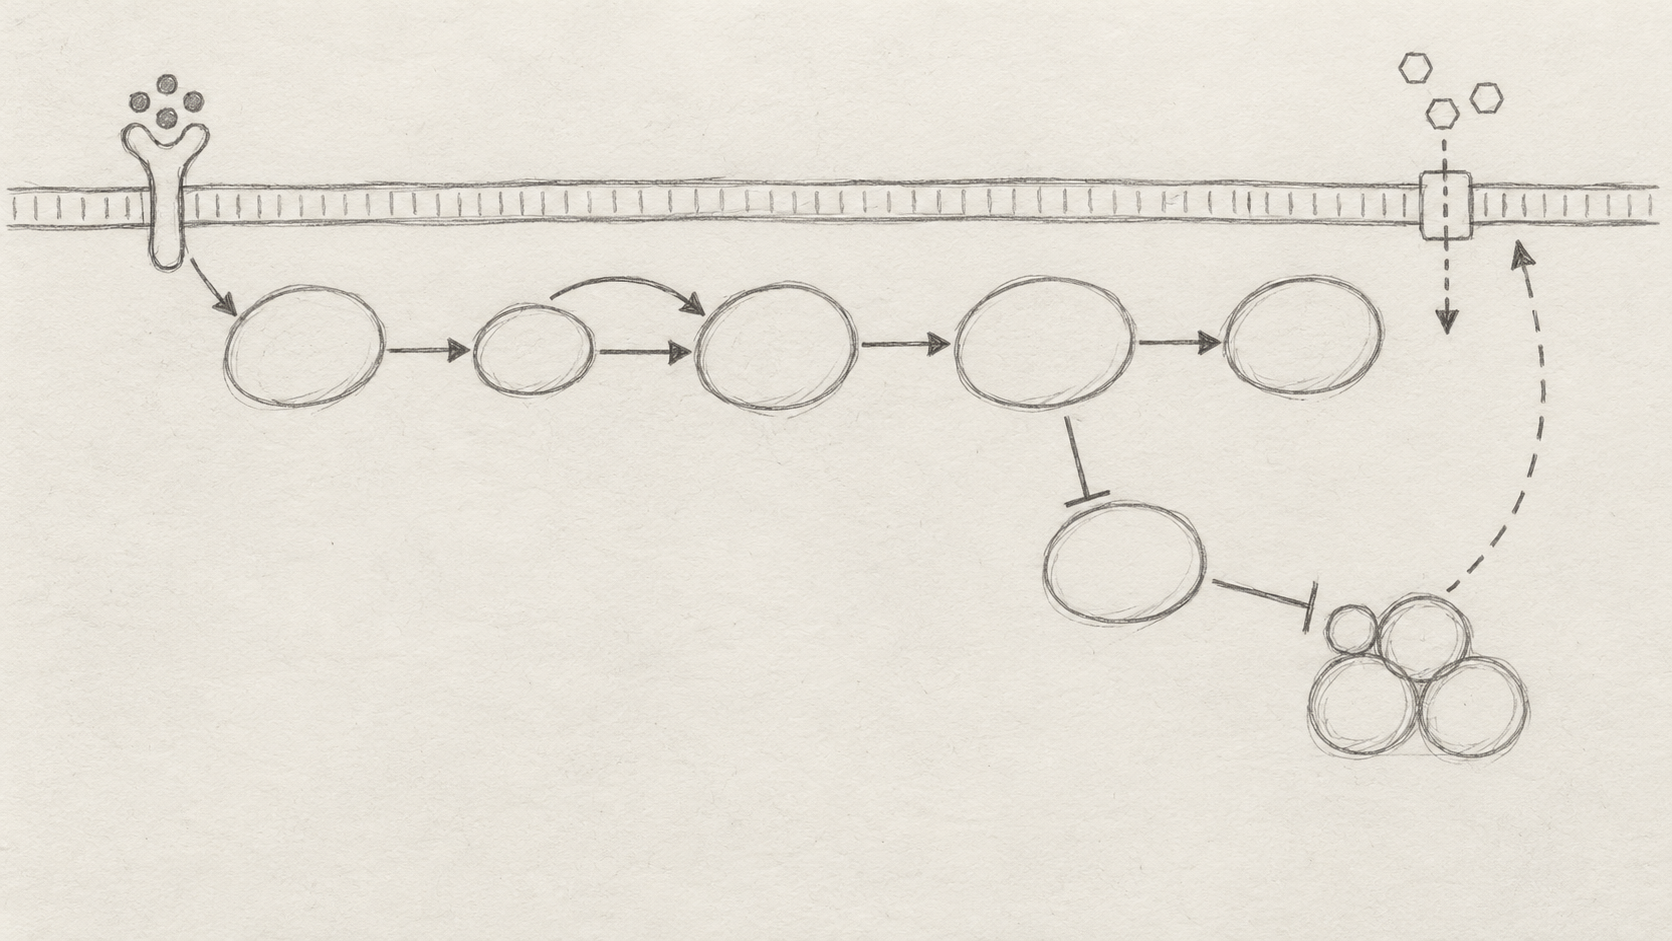
\includegraphics[width=\linewidth]{figures/ch07/ch07-02-v0-sketch.png}};
  \begin{scope}[x={(img.south east)}, y={(img.north west)}]
    \node at (0.12, 1-0.10) {\chsevenrelmark{1}};
    \node at (0.12, 1-0.28) {\chsevenrelmark{2}};
    \node at (0.17, 1-0.44) {\chsevenrelmark{3}};
    \node at (0.25, 1-0.42) {\chsevenrelmark{4}};
    \node at (0.37, 1-0.26) {\chsevenrelmark{5}};
    \node at (0.47, 1-0.37) {\chsevenrelmark{7}};
    \node at (0.53, 1-0.50) {\chsevenrelmark{8}};
    \node at (0.58, 1-0.46) {\chsevenrelmark{9}};
    \node at (0.67, 1-0.58) {\chsevenrelmark{10}};
    \node at (0.80, 1-0.45) {\chsevenrelmark{11}};
    \node at (0.87, 1-0.24) {\chsevenrelmark{12}};
    \node at (0.88, 1-0.12) {\chsevenrelmark{13}};
    \node at (0.44, 1-0.36) {\chsevenrelmark{6}};
  \end{scope}
\end{tikzpicture}

\caption{根据关系表安排布局的手绘草图（图像模型模拟的铅笔草图，非真实手稿）。圆圈编号对应表~\ref{tab:ch07-01} 的关系 R1–R13。草图只确定分区、对象大致位置与阅读路径，不承担对象名称；以草图作为生成输入时，它是布局意图而非布局锁定。}\label{fig:ch07-02}
\end{figure}

图~\ref{fig:ch07-02} 的底图由图像模型模拟铅笔草图生成，圆圈编号 ①–⑬ 在排版阶段用 TikZ 叠加。即便只是生成这样一张构图草图，把同一段提示词连续生成三次，前两次结果都只画了一条 T 形抑制线，且把右下方的囊泡节点与主链断开；第三次生成时专门追加了“必须画出两条串联 T 形抑制线连至囊泡表面小珠”的指令，才得到图~\ref{fig:ch07-02} 中 ⑨ 与 ⑩ 串联的结构。但与此同时，模型把 Akt 下方原本向上指的 mTORC2 团块省去了，反而在主链右侧多画了一个团块；右侧葡萄糖穿膜线（⑬）也画成了短虚线而非点线，左侧配体圆点（①）与受体之间留有小隙。

这正好说明草图的定位：草图不写分子名，只帮作者和工具理顺空间分区与流向。在 SciDraw AI 中，作者可把草图上传至“草图模式”，配合文字任务书生成初稿。但草图约束只是构图意图，不等于硬性的“对象锁定”或布局保持，生成后仍须按表~\ref{tab:ch07-01} 逐行核查。

\section{一句话提示词为什么不够}

为了对比输入完整度对结果的决定性影响，我们把开篇的一句话提示词（V1）与完整任务书驱动的提示词（V2）放进同一环境，并排检验实际产出（图~\ref{fig:ch07-03}）。

在 SciDraw AI 中，建议先打开科研绘图向导（\sdtool{figure-workflow}），选择“机制图与流程图”路线，把默认任务书替换为结构化任务书并下载副本，再进入机制图生成（\sdtool{mechanism-figure-generator}）或提示词绘图（\sdtool{ai-drawing}）。向导只负责组织任务书和串联工具，不会自动检查科学关系。本案例任务书的关键部分如下（完整提示词见本书仓库 \texttt{cases/} 目录）：

\begin{Prompt}
【用途与目标】论文 Figure 1 背景机制图（双栏宽 174 mm）；交代胰岛素经 IR → IRS-1 →
PI3K → PIP3 → Akt 的级联、Akt ⊣ AS160 ⊣ Rab 的双重抑制，以及 GSV 转位融合与葡萄糖内流。
【对象与计数】每个对象只出现一次（GLUT4 除外）：胞外为胰岛素、葡萄糖；质膜为脂双层、
胰岛素受体、内叶 PIP2/PIP3、膜上 GLUT4；胞质为 IRS-1、PI3K、PDK1、Akt、mTORC2、
AS160、囊泡表面 Rab、嵌有 GLUT4 的储存囊泡簇（GSV）。受体、IRS-1、Akt、AS160 标磷酸化圆点。
【关系与线型】R1 胰岛素接触受体（无箭头）；R2 受体自身磷酸化（2 圆点）；R3 受体 → IRS-1、
R4 IRS-1 → PI3K、R7 PDK1 → Akt、R8 mTORC2 → Akt 均为实线实心激活箭头（mTORC2 无上游线）；
R5 PI3K 催化 PIP2 → PIP3 为细弧空心 V 头（PI3K 短线触弧中点）；R6 PIP3 贴膜招募 PDK1 与 Akt；
R9 Akt ⊣ AS160、R10 AS160 ⊣ Rab 均为 T 形抑制线；R11–R12 GSV 向质膜 GLUT4 转位融合为
橙色粗虚线空心箭头；R13 葡萄糖穿过膜 GLUT4 进入胞质为深橙点线箭头。
【布局与视觉】16:9 横幅；上方 20% 胞外、20–28% 质膜、下方胞质、底部 10% 留空给图例。
白底扁平二维矢量风格，无渐变、阴影或 3D；信号蛋白中等蓝，AS160/Rab 灰蓝，GLUT4/GSV/葡萄糖
柔和橙色，膜浅暖灰，磷酸化琥珀色圆点。
【限制】底图不出现任何文字、字母或数字；不画细胞核、内质网、细胞骨架或 MAPK 等旁路。
\end{Prompt}

反例 V1 提交的英文提示词只有一句话：

\begin{Prompt}
Make a beautiful, professional scientific illustration of insulin signaling and
GLUT4 translocation for a top journal.
\end{Prompt}

正例初稿 V2 则将任务书转为结构化英文提示词，明确空间比例（\texttt{SPACE}）、十三个对象的形状与位置（\texttt{OBJECTS}）、五种线型（\texttt{RELATIONS}）和禁画清单（\texttt{DO NOT DRAW}），并要求全图无任何文字（完整提示词见本书仓库 \texttt{cases/} 目录，关键部分如下）：

\begin{Prompt}
Flat 2D scientific schematic for a journal figure, landscape 16:9, pure white
background. Clean vector style, flat fills, thin dark outlines, no gradients,
no shadows, no 3D. ABSOLUTELY NO TEXT: no letters, words, numbers, or symbols.
SPACE: Top 20% = extracellular; 20-28% = horizontal lipid bilayer membrane;
28-88% = cytoplasm; bottom 12% = empty white strip reserved for legend.
OBJECTS (each appears once; GLUT4 appears in vesicles and in plasma membrane):
1. Insulin (3 dark-blue beads touching receptor); 2. Transmembrane receptor (2 amber dots);
3. IRS-1 (1 amber dot); 4. PI3K; 5. Inner-leaflet PIP2 & PIP3; 6. PDK1 & 7. Akt
   (both touching inner leaflet at PIP3; Akt has 2 amber dots); 8. mTORC2 below Akt;
9. AS160 (gray-blue, 1 amber dot); 10. GSV cluster (3 vesicles with orange GLUT4 barrels);
11. Rab bead on vesicle; 12. GLUT4 in right plasma membrane; 13. Glucose hexagons above it.
RELATIONS (draw only these):
- Activation (solid dark-gray line, filled triangle): IR -> IRS-1 -> PI3K; PDK1 -> Akt; mTORC2 -> Akt.
- Inhibition (solid dark-gray line, perpendicular T-bar): Akt -| AS160; AS160 -| Rab.
- Enzymatic conversion (thin mid-gray arc, open V head): PIP2 -> PIP3, PI3K stub touching midpoint.
- Translocation (thick dashed orange arrow, open head): GSV cluster upward to membrane GLUT4.
- Substance flow (dotted dark-orange arrow): extracellular glucose through membrane GLUT4 into cell.
\end{Prompt}

\begin{figure}[htbp]\centering
% FIG ch07-03a V1 error markers (language-neutral)
\definecolor{ch07err}{HTML}{C0392B}
\makeatletter
\@ifundefined{chsevenerrmark}{%
\newcommand{\chsevenerrmark}[2][]{%
  \tikz[baseline=(char.base)]{%
    \node[shape=circle, fill=ch07err, text=white, inner sep=1.5pt,
      font=\fontsize{7}{7}\selectfont\bfseries, #1] (char) {#2};}}%
}{}
\makeatother
\begin{tikzpicture}
  \node[anchor=south west, inner sep=0] (img) at (0,0)
    {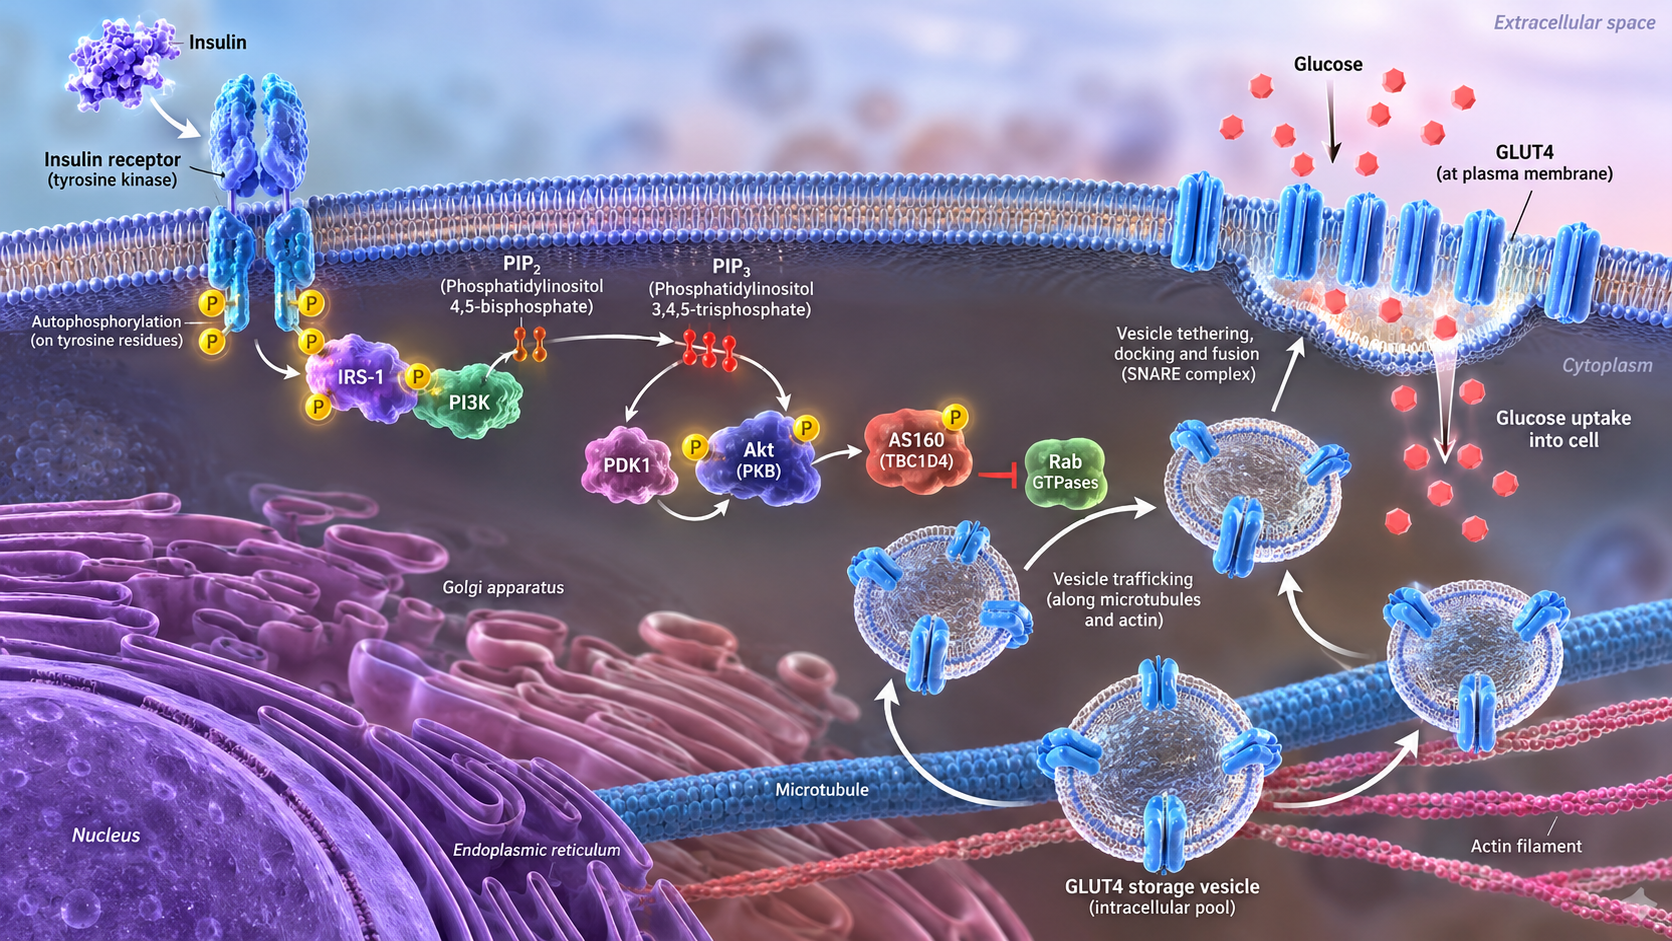
\includegraphics[width=\linewidth]{figures/ch07/ch07-03a-v1-vague.png}};
  \begin{scope}[x={(img.south east)}, y={(img.north west)}]
    \node at (0.14, 1-0.18) {\chsevenerrmark{1}};
    \node at (0.72, 1-0.22) {\chsevenerrmark{2}};
    \node at (0.50, 1-0.35) {\chsevenerrmark{3}};
    \node at (0.38, 1-0.55) {\chsevenerrmark{4}};
    \node at (0.55, 1-0.72) {\chsevenerrmark{5}};
    \node at (0.22, 1-0.48) {\chsevenerrmark{6}};
    \node at (0.82, 1-0.40) {\chsevenerrmark{7}};
  \end{scope}
\end{tikzpicture}


\vspace{2mm}
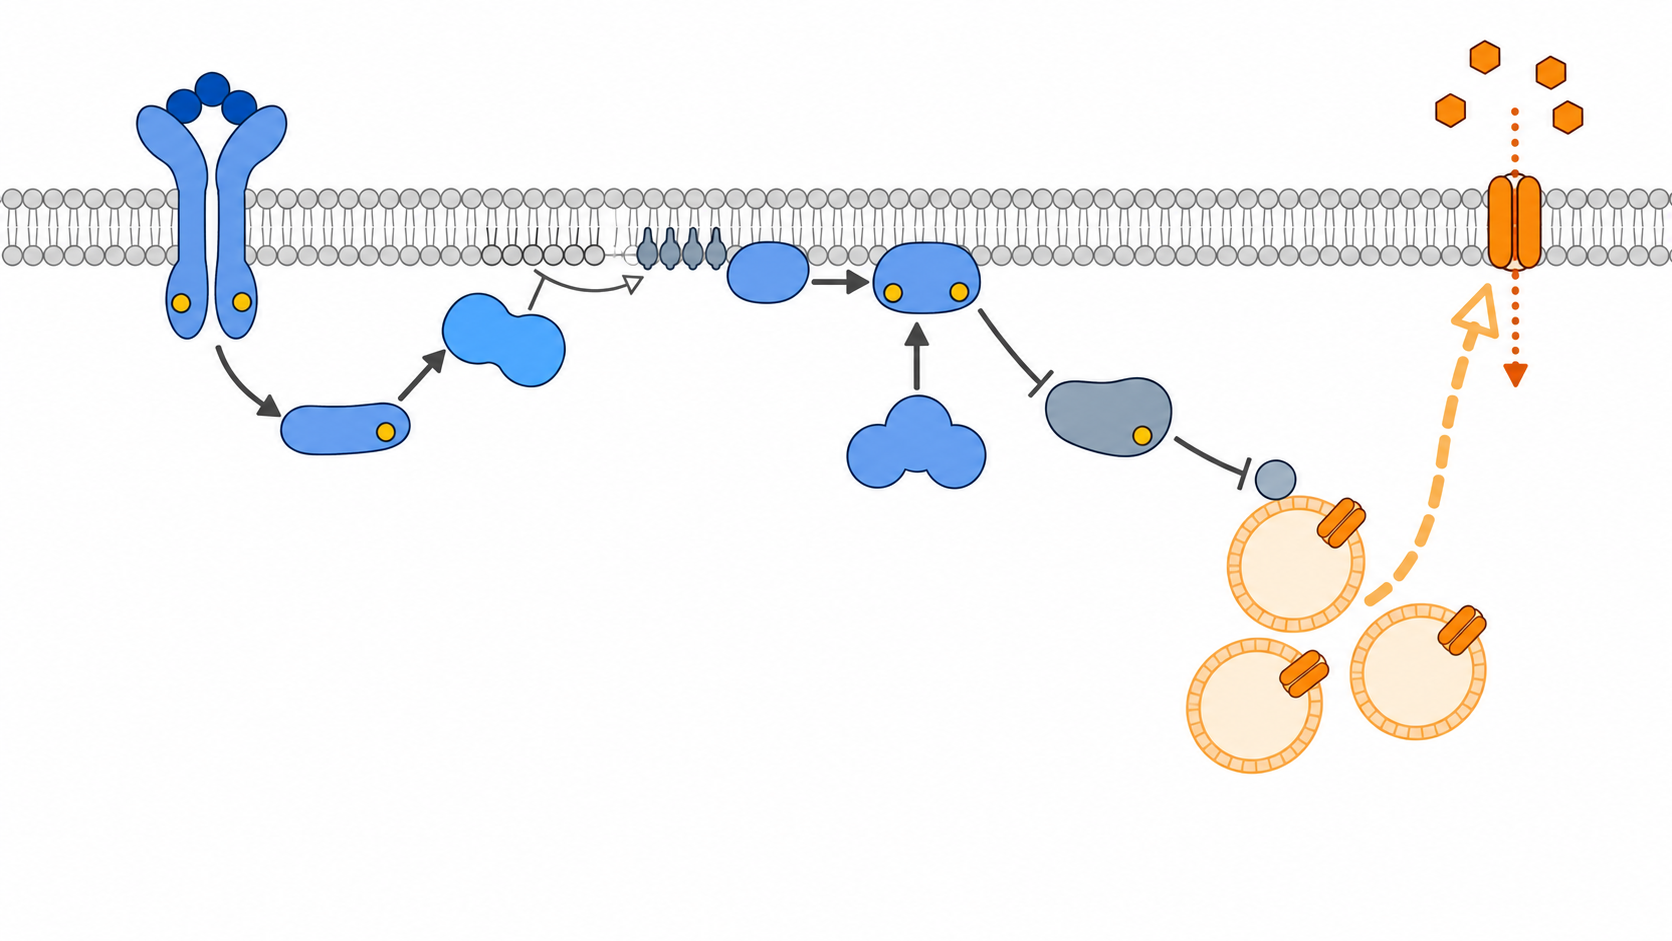
\includegraphics[width=\linewidth]{figures/ch07/ch07-03b-v2-brief.png}
\caption{一句话提示词与完整任务书的生成结果对照。（a）只用一句话提示词生成的初稿；模型把文字直接烤入深色背景，红色编号对应正文列出的问题。（b）使用完整任务书生成的无字初稿：对象与关系基本可逐条核对，配色、线宽与留白尚未统一。本章示例图由图像模型生成，提示词与生成记录见本书仓库。}\label{fig:ch07-03}
\end{figure}

检查图~\ref{fig:ch07-03}a 时可以看到：模型不仅直接把英文标签烤进了位图，而且在缩至 174 mm 通栏印刷宽度后，深色三维背景与发光特效上的小字难以辨认，后期也无法单独调整字号或改正拼写。更重要的是，对照表~\ref{tab:ch07-01} 逐项核查，这张看似华丽的初稿存在七处明显问题（对应图~\ref{fig:ch07-03}a 的红色编号 ❶–❼）：
\begin{enumerate}
\item \textbf{配体结合方式与 3D 装饰过度（❶）：} 胞外胰岛素到受体画了白色箭头而非直接接触（违反 R1）；蛋白带强烈高光、阴影与发光“P”球，干扰边界识别。
\item \textbf{膜上对象重复与文字堆砌（❷）：} 右上质膜凹坑内并排塞进六个蓝色 GLUT4 通道（违反唯一计数），并在胞质中印上三行关于 SNARE 的描述性文字。
\item \textbf{核心关系反转、缺支路与位置错误（❸）：} 首先，\textbf{mTORC2 完全缺失}（缺 R8）。其次，\textbf{Akt 到 AS160 被画成白色实心激活箭头}（R9 错误），而 AS160 到 Rab 画了红色 T 形抑制线（R10）——串起来读竟变成“Akt 激活 AS160 进而抑制 Rab”，与生物学事实完全相反！此外，$\text{PIP}_3$ 用箭头连向远离质膜的 PDK1 与 Akt（违反 R6 贴膜要求），绿色的 Rab 游离在胞质中而未附着囊泡表面。
\item \textbf{无关细胞器占据半幅画面（❹）：} 左下绘出巨大的细胞核、内质网和高尔基体，挤占了信号主干空间。
\item \textbf{细胞骨架与循环弯箭头造成歧义（❺）：} 右下画出微管与肌动蛋白丝，四个剖面囊泡由弯箭头连成环路，分不清储存池与转位方向。
\item \textbf{上游蛋白重叠与催化连接错误（❻）：} IRS-1 与 PI3K 直接重叠，缺少激活箭头（R4 不清）；PI3K 指向 $\text{PIP}_2$ 本身而非转化弧中点（R5 错误）。
\item \textbf{箭头同型且无图例（❼）：} 除一处红 T 端外，结合、催化、激活、囊泡移动和葡萄糖内流全用白色实心箭头，且无图例。
\end{enumerate}

为什么 Akt 抑制 AS160（R9）与 AS160 抑制 Rab（R10）这段“抑制的抑制”必须保留两条串联 T 形线？基础状态下，AS160 具有 GAP 活性，促使 Rab 水解 GTP 变为失活态，像刹车一样把囊泡扣留在胞质（Sano 等，2003；Leto 与 Saltiel，2012）。Akt 磷酸化并\textbf{抑制} AS160，相当于松开刹车，使 Rab 维持 GTP 结合态并推动囊泡转位。如果省成“Akt $\rightarrow$ GSV”一条大箭头，就抹去了可核对的机制节点；如果像图~\ref{fig:ch07-03}a 那样画成一激活一抑制，则直接画反了因果。

再看按完整任务书生成的图~\ref{fig:ch07-03}b。把同一提示词生成两次时，第一张候选图曾把本应指向 AS160 的 T 形线错接到 mTORC2 上，并在囊泡表面画了两颗 Rab 珠；第二张候选图（图~\ref{fig:ch07-03}b）纠正了这一连接。图中“胞外—质膜—胞质”三分区清楚，十三个对象计数、六枚琥珀色磷酸化圆点及五类线型全部到位，无多余细胞器或文字。这证明结构正确主要取决于输入任务书的完整度，同时每次生成仍须逐条核对连接点。

\section{线型与颜色：只让它们承担一种含义}

拿到结构初稿后，修改阶段最容易出现两类偏差：一是随意变换箭头的线型、粗细和颜色；二是给每个蛋白涂上高饱和度的不同颜色。下面通过两组对照图说明视觉规范。

第一组对照（图~\ref{fig:ch07-04}）截取“Akt $\dashv$ AS160 $\dashv$ Rab $\rightarrow$ 囊泡转位至膜 GLUT4”局部。图~\ref{fig:ch07-04}a 故意混用四种线：蓝椭圆到灰蓝团块用粗红实心弯箭头（把抑制画成激活），灰蓝团块到囊泡小珠用细绿虚线空心头，囊泡簇到膜转运体用与普通激活相同的黑色实线实心箭头（让人误以为囊泡“激活”了 GLUT4），蓝椭圆与质膜间还多出一条含义不明的紫色双向箭头。图~\ref{fig:ch07-04}b 则只用三条线、两种线型：两条等粗深灰 T 形线串联表示双重抑制，唯一一条柔和橙色粗虚线空心头向上表示空间转位（放大检查仍可见 T 端留有微隙、蛋白带轻微渐变）。无需文字，读者也能从图~\ref{fig:ch07-04}b 区分负调控信号与空间移动。

\begin{figure}[htbp]\centering
\begin{minipage}[t]{0.48\linewidth}\centering
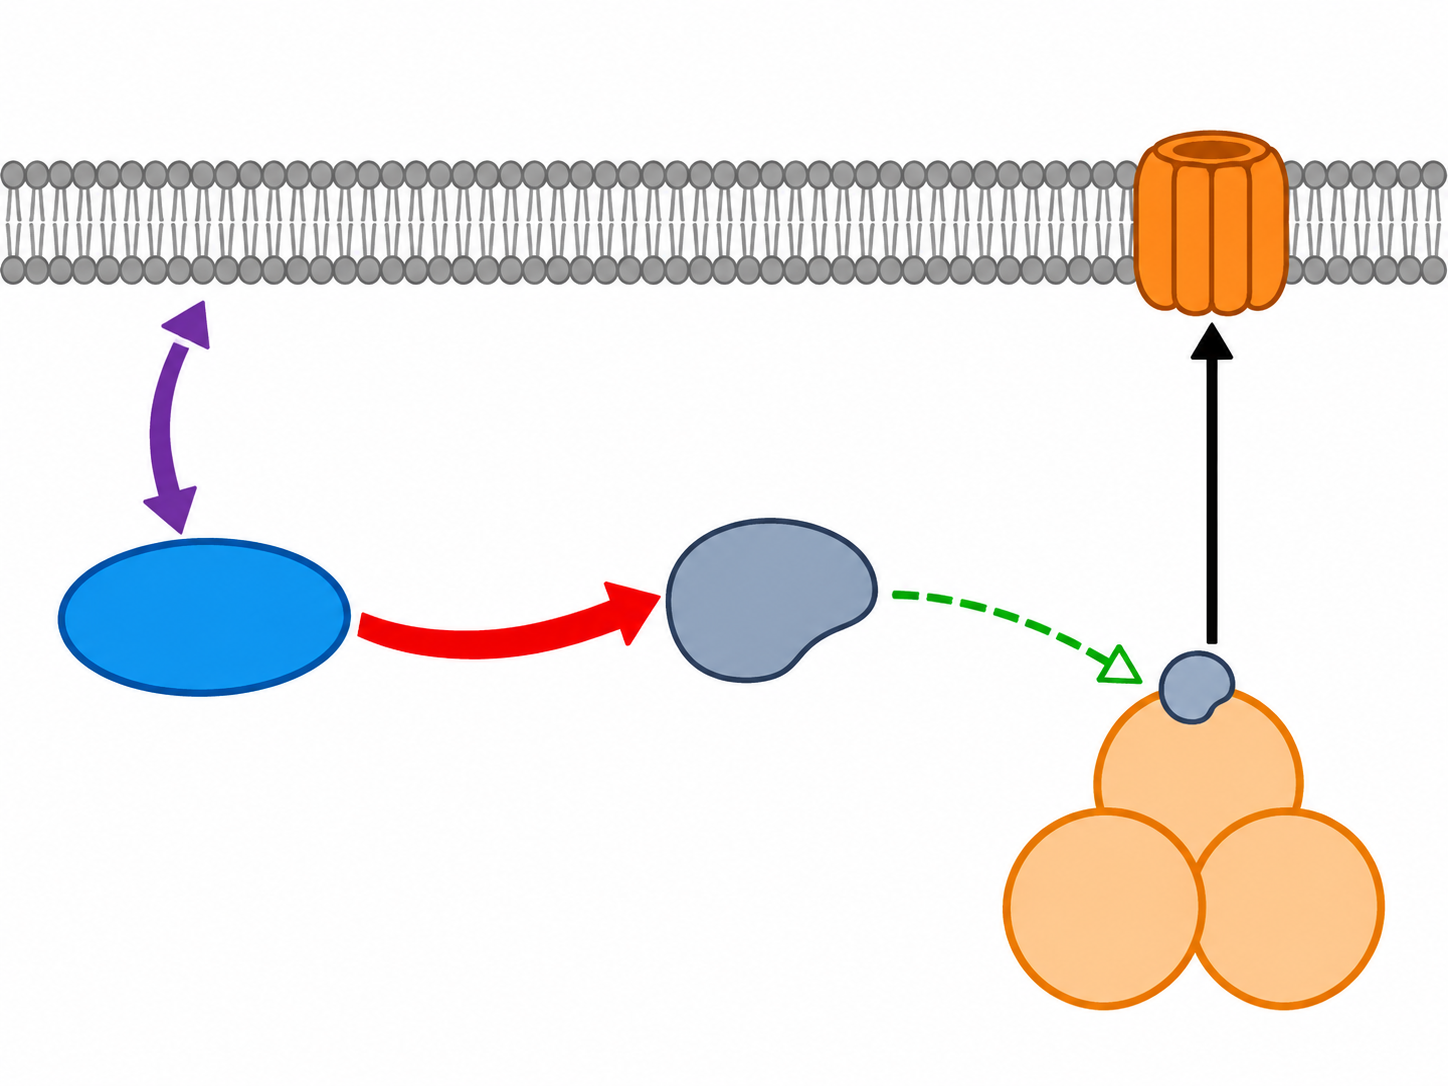
\includegraphics[width=\linewidth]{figures/ch07/ch07-04a-mixed-arrows.png}\\[1mm]
{\footnotesize (a) 线型混用：抑制、转位与双向箭头混淆}
\end{minipage}\hfill
\begin{minipage}[t]{0.48\linewidth}\centering
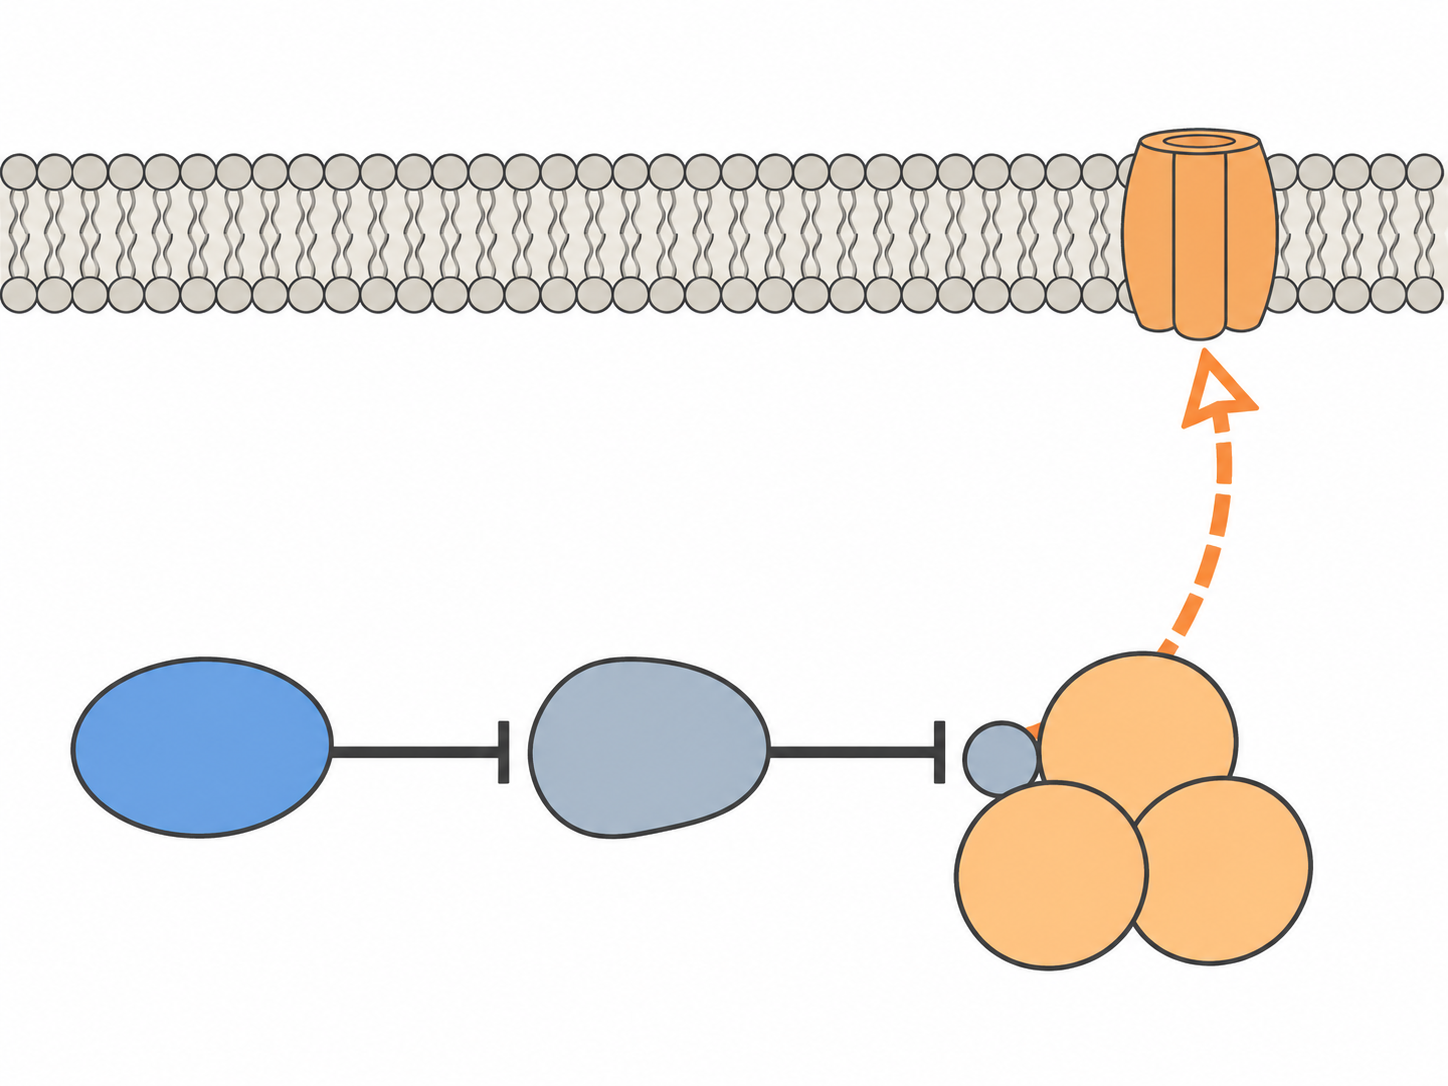
\includegraphics[width=\linewidth]{figures/ch07/ch07-04b-unified-arrows.png}\\[1mm]
{\footnotesize (b) 线型统一：两条串联 T 形线与粗虚线转位}
\end{minipage}
\caption{同一段简化通路的两种画法。（a）线型、颜色和粗细随意变化，转位箭头与激活箭头同型，另有一条含义不明的双向箭头。（b）两条 T 形线串联表示“抑制的抑制”，粗虚线是唯一的空间转位符号。}\label{fig:ch07-04}
\end{figure}

第二组对照（图~\ref{fig:ch07-05}）比较配色过多与配色克制，并展示灰度测试结果。

\begin{figure}[htbp]\centering
\begin{minipage}[t]{0.48\linewidth}\centering
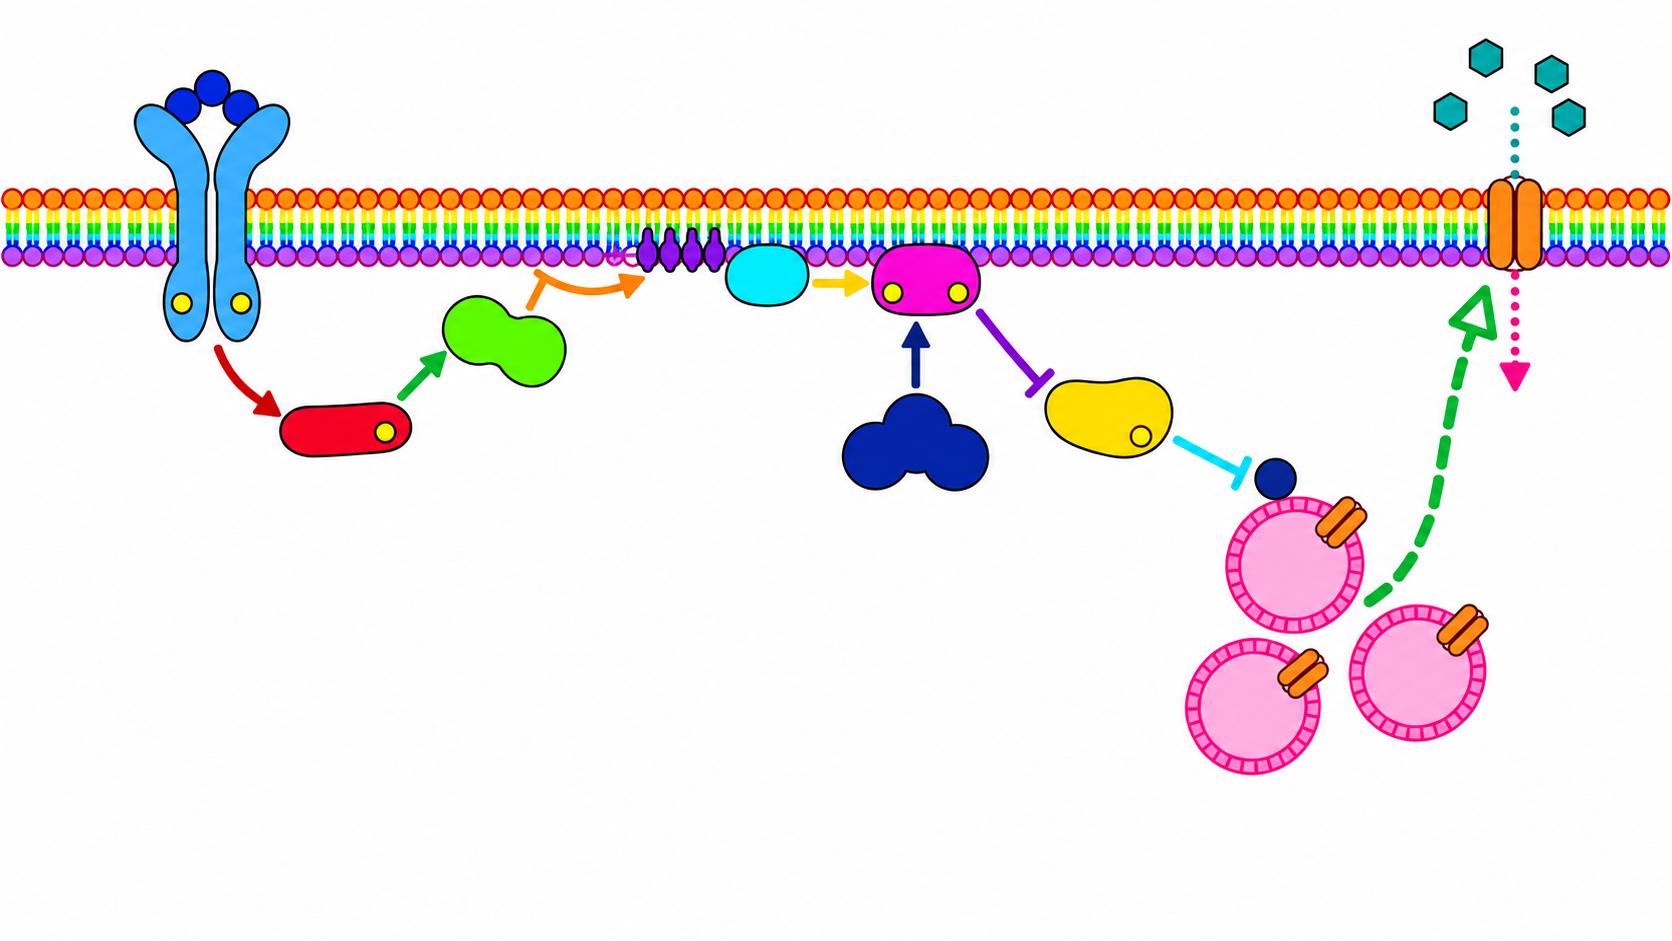
\includegraphics[width=\linewidth]{figures/ch07/ch07-05a-many-colours.png}\\[1mm]
{\footnotesize (a) 配色过多：每蛋白异色与彩虹膜}
\end{minipage}\hfill
\begin{minipage}[t]{0.48\linewidth}\centering
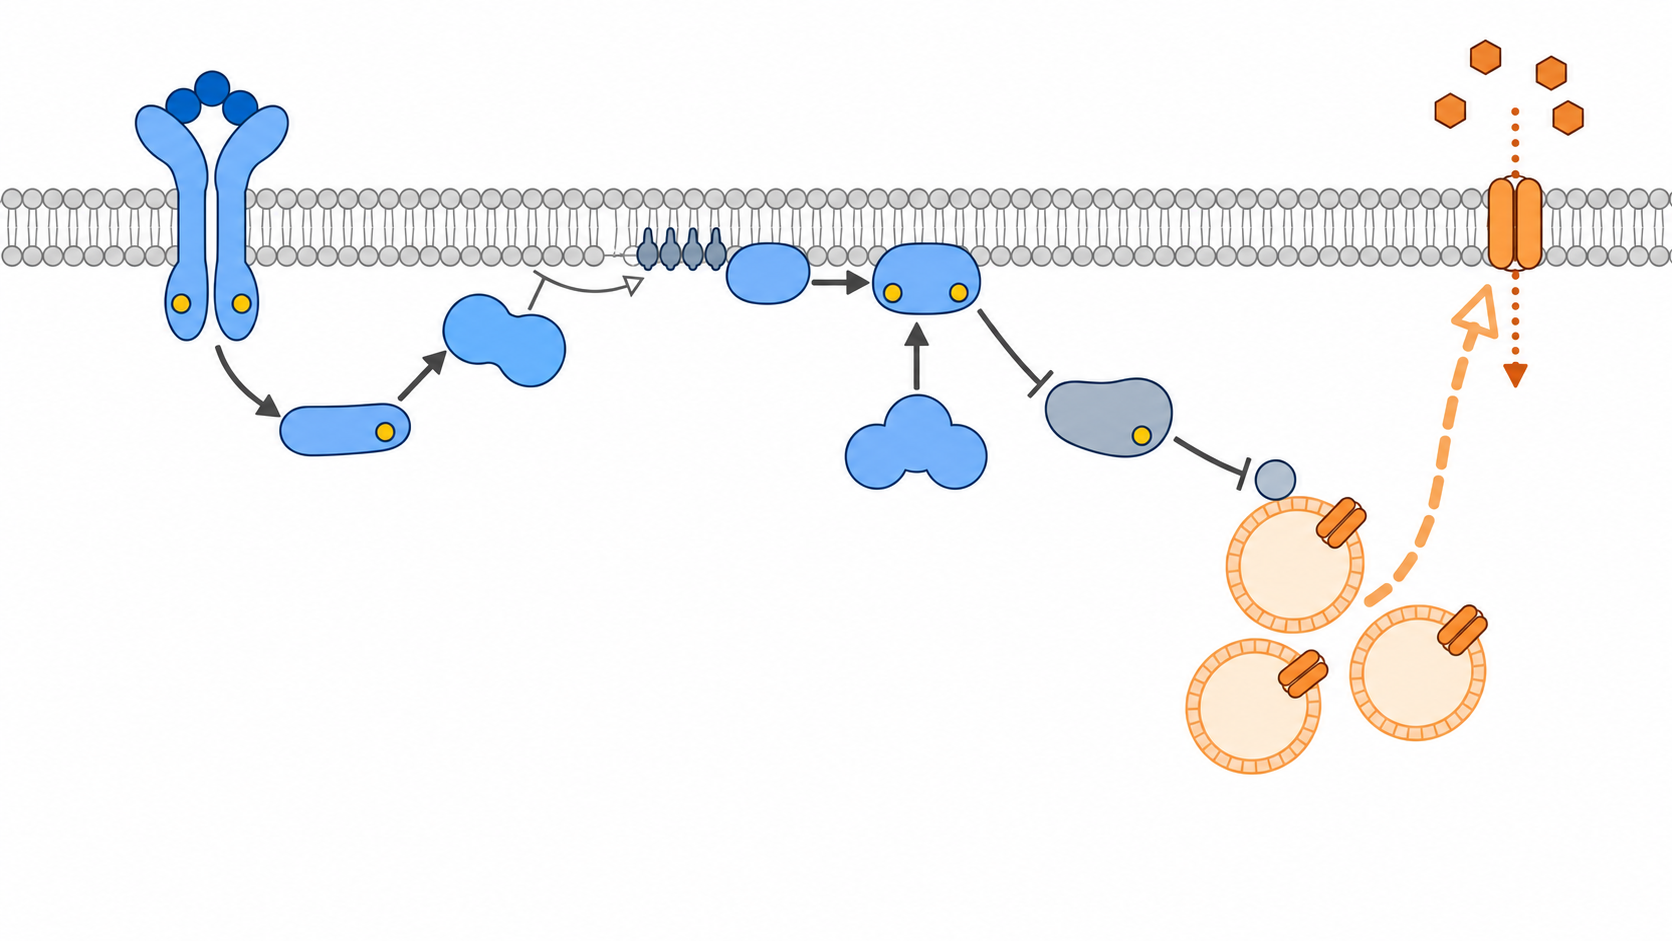
\includegraphics[width=\linewidth]{figures/ch07/ch07-05b-v3-revised.png}\\[1mm]
{\footnotesize (b) 配色克制（V3）：三种角色色相加灰}
\end{minipage}

\vspace{2mm}
\begin{minipage}[t]{0.48\linewidth}\centering
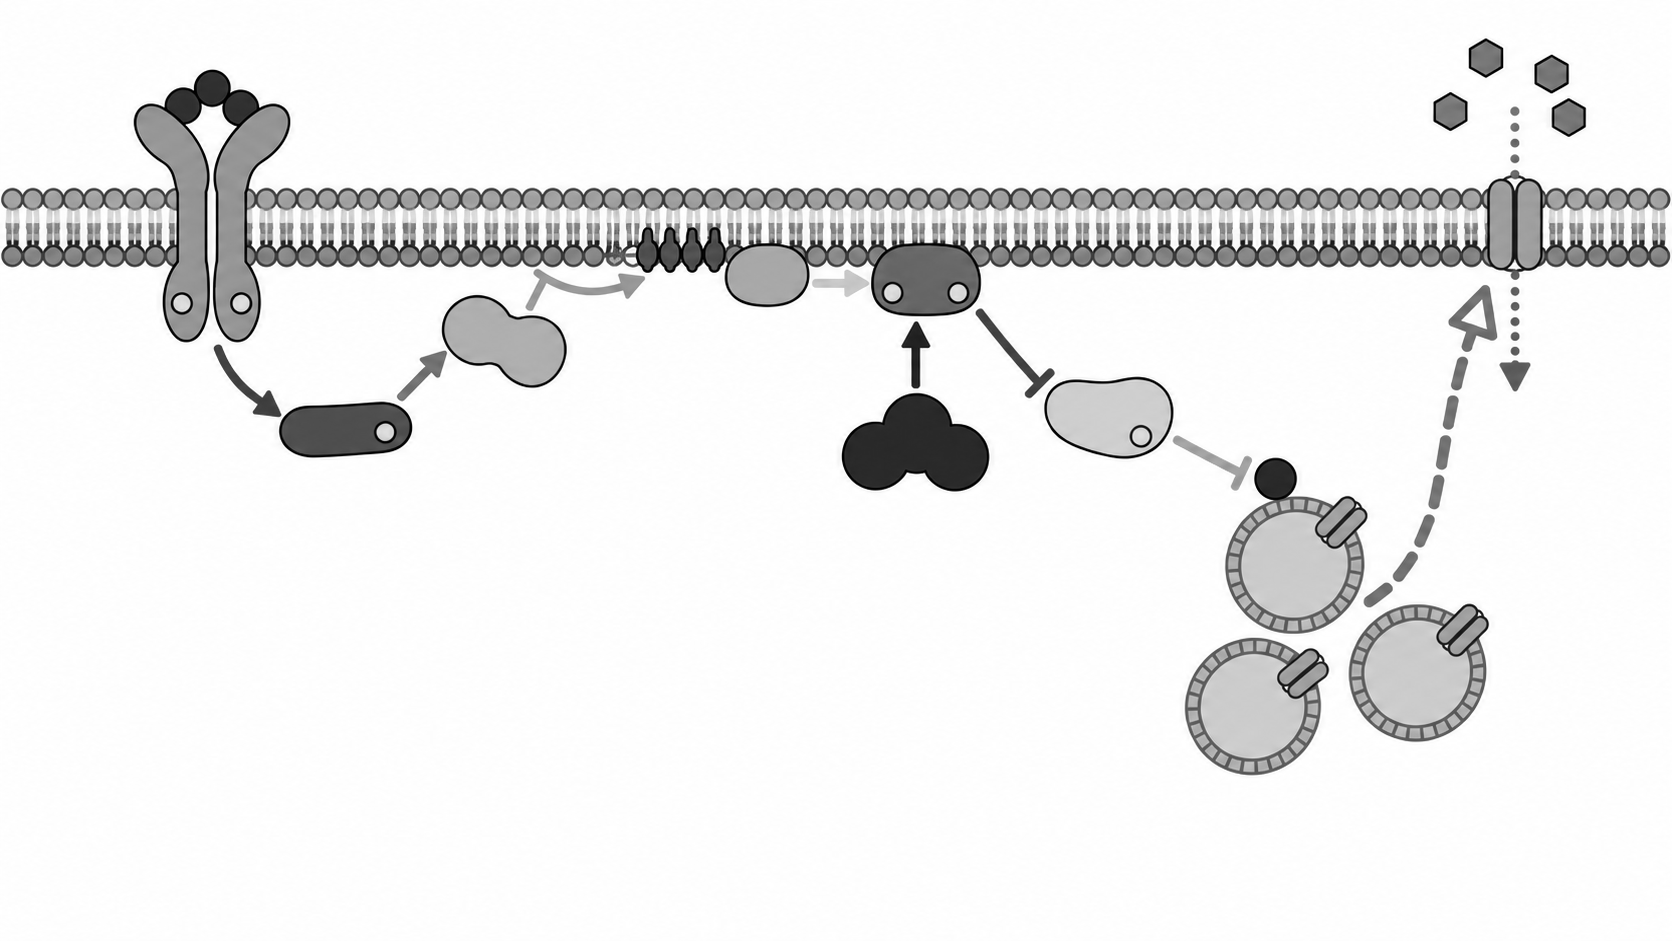
\includegraphics[width=\linewidth]{figures/ch07/ch07-05a-many-colours-gray.png}\\[1mm]
{\footnotesize (c) 图 (a) 的灰度转换结果}
\end{minipage}\hfill
\begin{minipage}[t]{0.48\linewidth}\centering
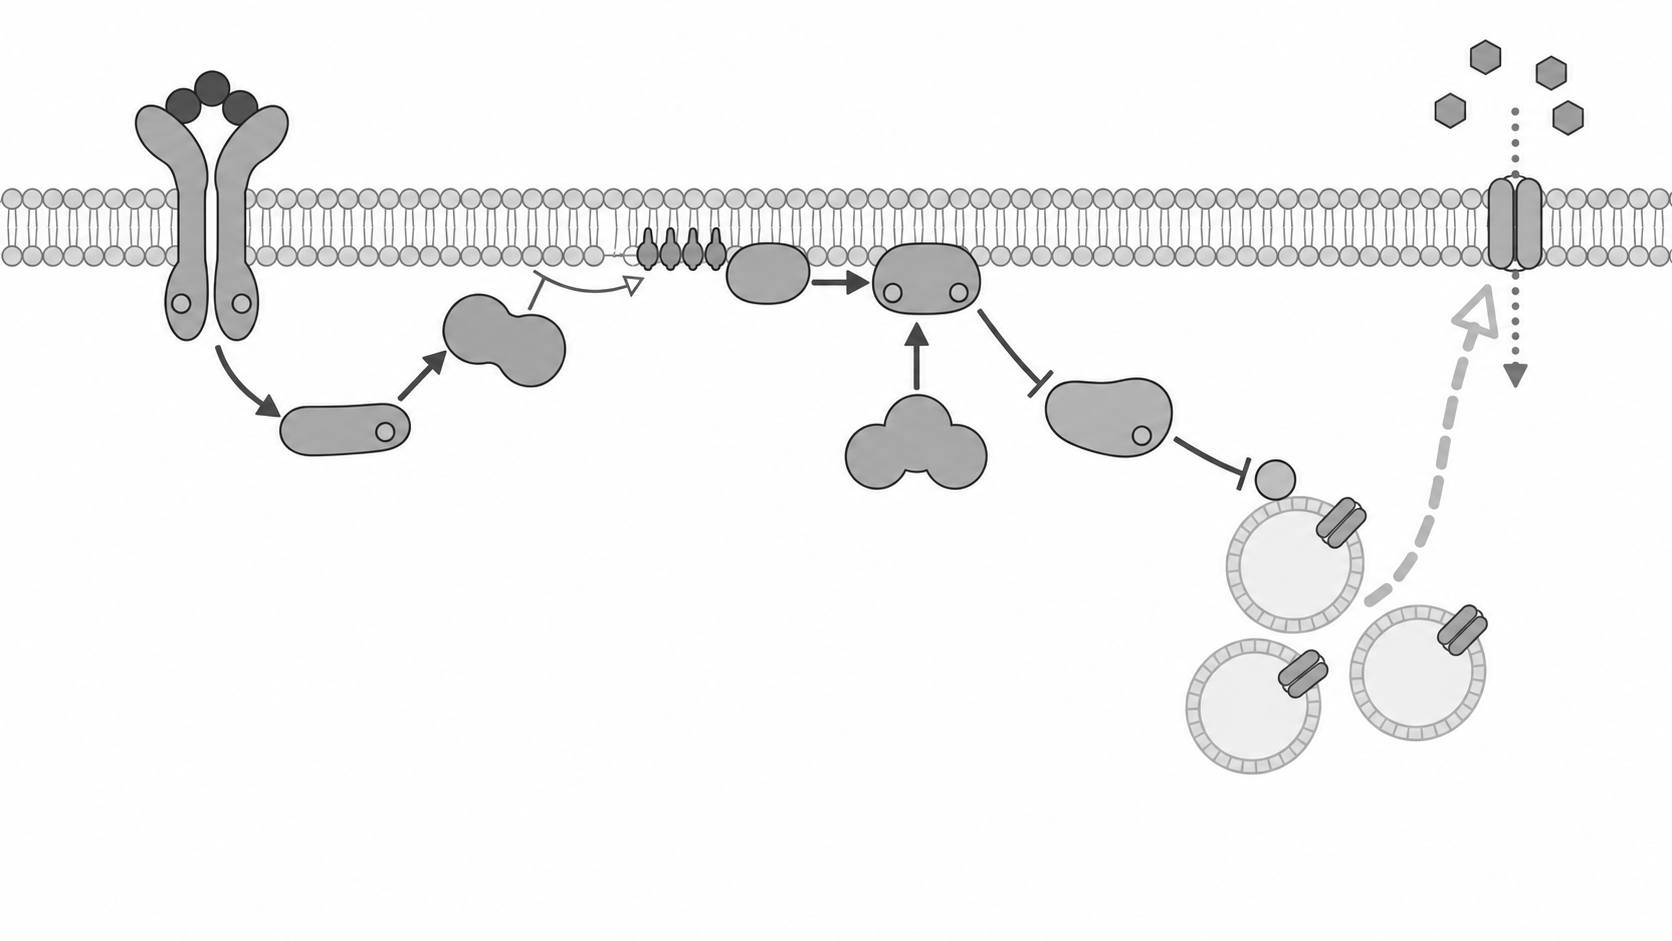
\includegraphics[width=\linewidth]{figures/ch07/ch07-05b-v3-revised-gray.png}\\[1mm]
{\footnotesize (d) 图 (b) 的灰度转换结果}
\end{minipage}
\caption{机制图的配色对比与灰度测试。（a）每个蛋白一种饱和色、彩虹色膜，颜色不承担含义。（b）修订稿（V3）只用三种色相加灰色，分别对应信号蛋白、运输调控蛋白、运输物质及其载体。下行为两图的灰度版本：（b）的层级与线型在灰度下仍可辨认。}\label{fig:ch07-05}
\end{figure}

生成图~\ref{fig:ch07-05}a 的过程同样说明了模型的不稳定性：第一次在不带参考图的情况下要求“每个蛋白涂不同颜色、质膜涂成彩虹色”时，模型为了迎合花哨配色，竟把整条通路改写成了单条六蛋白激活链，丢掉了两条 T 形抑制线和 mTORC2，还把葡萄糖跨膜箭头画反；第二次以图~\ref{fig:ch07-05}b 作参考图才保住主体布局，但 $\text{PIP}_2 \rightarrow \text{PIP}_3$ 转化弧的箭头仍意外由空心变成了实心。

对比图~\ref{fig:ch07-05}a 与 b 可以看出三点原则（Rougier 等，2014；Wong，2011）：第一，颜色应只编码功能角色。图~\ref{fig:ch07-05}a 中蛋白涂成红、亮绿、青、洋红、深蓝、明黄，读者找不到分组依据（如 mTORC2 与 Rab 同为深蓝却无关联）；图~\ref{fig:ch07-05}b 则只用三个色相——正向信号蛋白统一中等蓝，负调控与运输开关（AS160、Rab）统一低饱和灰蓝，被转运物质与载体（葡萄糖、GLUT4、囊泡）统一柔和橙色，质膜用浅暖灰。第二，避免红绿并用。图~\ref{fig:ch07-05}a 中红绿蛋白与红绿箭头相邻，对红绿色觉差异读者不友好（Wong，2011；选色可借助 ColorBrewer 2.0）。第三，通过灰度测试检验层级。将彩图转为灰度后，图~\ref{fig:ch07-05}c 的彩虹膜沉重刺眼、各蛋白明度杂乱；而图~\ref{fig:ch07-05}d 中同类蛋白明度一致，五种线型依靠实线、T 端、细弧、粗虚线和点线的几何形状依然可辨（同时可见橙色粗虚线转灰后偏浅，提示终稿可在虚线旁加文字辅助）。作者可用 SciDraw AI 的“图片检查”（\sdtool{figure-checker}）检查灰度与色觉风险，但须知它只是技术检查，无法判断科学关系正误。

\section{主案例：从修订到终稿}

下面梳理主案例从 V2 初稿（图~\ref{fig:ch07-03}b）到 V3 修订稿（图~\ref{fig:ch07-05}b）、再到 V4 终稿（图~\ref{fig:ch07-06}）、图注与核验的完整闭环。

\subsection{从 V2 到 V3：修改指令与“意外变化”的拦截}

对照表~\ref{tab:ch07-01} 核查 V2 初稿（图~\ref{fig:ch07-03}b），其主干拓扑与对象数正确，但放大检查仍可见五处具体偏差：（1）PI3K 催化 $\text{PIP}_2 \rightarrow \text{PIP}_3$ 的转化弧（R5）画成了闭合空心三角头而非开放 V 头，且 PI3K 催化短线接在弧线左端而非中点；（2）膜招募环节（R6）中 Akt 离质膜内叶 $\text{PIP}_3$ 头基稍远；（3）双重抑制环节（R9、R10）的 T 形端与靶标之间、以及囊泡转位箭头终点（R12）与膜上 GLUT4 之间留有窄白隙；（4）蛋白填充仍有轻微明暗渐变；（5）局部留白偏紧，直接叠加文字容易压住图形边缘，且底图在 174 mm 通栏宽度下折算分辨率约 244 ppi，尚未达到期刊常见的 300 ppi 印刷要求。

推进到 V3 时，修改指令先写“保持不变”的部分，再逐条写可核对的改动：

\begin{Prompt}
保持所有对象、位置和 13 条关系不变，只做以下修改：
1. 全部信号蛋白（受体、IRS-1、PI3K、PDK1、Akt、mTORC2）改为同一种中等蓝填充、同一深灰描边；
   AS160 与 Rab 改为同一种低饱和灰蓝。
2. 所有激活箭头与抑制线统一为同一粗细；抑制端统一为垂直短横线并紧贴靶标轮廓。
3. 酶促转化弧线改细、改为中灰开放 V 形头，PI3K 短线接触弧线中点，与激活箭头明显区分。
4. 胰岛素与葡萄糖保持约为蛋白的 1/3；GSV 簇清晰可辨。
5. 每个对象四周留出至少一个对象宽度的空白；底部 12% 清空；全图无任何文字。
\end{Prompt}

生成 V3 的两次尝试给出了关于“意外变化”的重要教训：第一次不带参考图直接按修订后的完整提示词重新生成时，模型弄丢了全部磷酸化圆点，把胰岛素减为 2 颗且脱离受体，让 PDK1 与 Akt 脱离质膜，在 PI3K 与 PDK1 之间凭空添了一条实心激活箭头，还把每个囊泡上的 GLUT4 画成了多个！第二次改以 V2 初稿作为参考图配合上述修改指令修订（得到图~\ref{fig:ch07-05}b），模型完整保住了十三个对象、六枚磷酸化点、贴膜关系与五类线型，未添多余箭头；代价是色彩明暗、PI3K 催化短线偏左与 T 端微隙改善有限。这说明：**每次修改后都必须重做全表复核，绝不能只看要求修改的那一处。**

\subsection{V4 终稿：无字底图加 LaTeX/TikZ 叠加层}

为什么终稿坚持“无字底图 + LaTeX/TikZ 叠加标签”？因为图像模型拼写分子名不可靠（如把 \texttt{Akt} 拼成 \texttt{Act} 即成科学错误），字号不可控，且每次生成位置漂移。把文字放到 TikZ 中，拼写可直接从清单复制，印刷字号精确控制在 7–8 pt，且中英文两版可以共用同一张无字底图，只需切换叠加层的语言文本。交付时可走\textbf{方案 A}（底图含对象与箭头，TikZ 只叠文字和图例，本例采用）或\textbf{方案 B}（底图只画对象，箭头也由 TikZ 绘制，下一节电池案例采用）。

以 V3 为参考生成 V4 底图时，提示词进一步锁定了色板与标签留白区（完整提示词见本书仓库 \texttt{cases/} 目录）：

\begin{Prompt}
Final base artwork for a journal Figure 1, flat 2D vector-style scientific
schematic, landscape 16:9, print resolution 300 ppi at 174 mm width, pure white
background, uniform thin dark gray (#3A3A3A) outlines, flat fills, no gradients.
THIS IMAGE MUST CONTAIN NO TEXT AT ALL: no letters, words, numbers, or "P".
PALETTE: signaling proteins #A9C4E0 / #4C78A8; insulin #2F5D8C; AS160 and Rab
#B8C2CC; GLUT4 and vesicles #F2C49B / #E39B5B; glucose #C46A2A; membrane
#D9D6D0 / #BDB8AF; phosphorylation dots #E3B23C; lines #3A3A3A and #7A7A7A.
LAYOUT & RELATIONS: keep the same 13 objects, phosphorylation dots, and 5 line
types as the reference image. Leave generous empty white margins above the
membrane, around each protein, and across the bottom 12% strip for overlaid
labels and the figure legend.
\end{Prompt}

生成 V4 底图时同样经历了从拦截偏差到排版微调的过程：第一次不带参考图生成时，模型曾把囊泡上的 GLUT4 错画进囊泡腔内；改用 V3 作参考图生成的第三次结果恢复了正确的囊泡膜嵌合位置，放大至 200\% 逐区检查确认无任何残余文字或水印。不过，模型生成的图形边缘仍占用了部分预留给文字的空白，PI3K 催化短线接点偏左与 T 形端微隙也依然存在，174 mm 通栏宽度下折算分辨率约 244 ppi。因此，在 LaTeX 中用 TikZ 建立以底图左下角为 $(0,0)$、右上角为 $(1,1)$ 的归一化坐标系后，我们根据底图实际留白微调了十七个标签的位置，在空间紧凑处用短引线避开图形边缘，并在底部空白带排版了矢量图例（图~\ref{fig:ch07-06}）。

\begin{figure}[htbp]\centering
% FIG ch07-06 GLUT4 final overlay (Chinese)
\definecolor{ch07comp}{HTML}{6B6B6B}
\definecolor{ch07transnote}{HTML}{C46A2A}
\definecolor{ch07act}{HTML}{3A3A3A}
\definecolor{ch07conv}{HTML}{7A7A7A}
\definecolor{ch07trans}{HTML}{E39B5B}
\definecolor{ch07flux}{HTML}{C46A2A}
\definecolor{ch07phos}{HTML}{E3B23C}
\begin{tikzpicture}
  \node[anchor=south west, inner sep=0] (img) at (0,0)
    {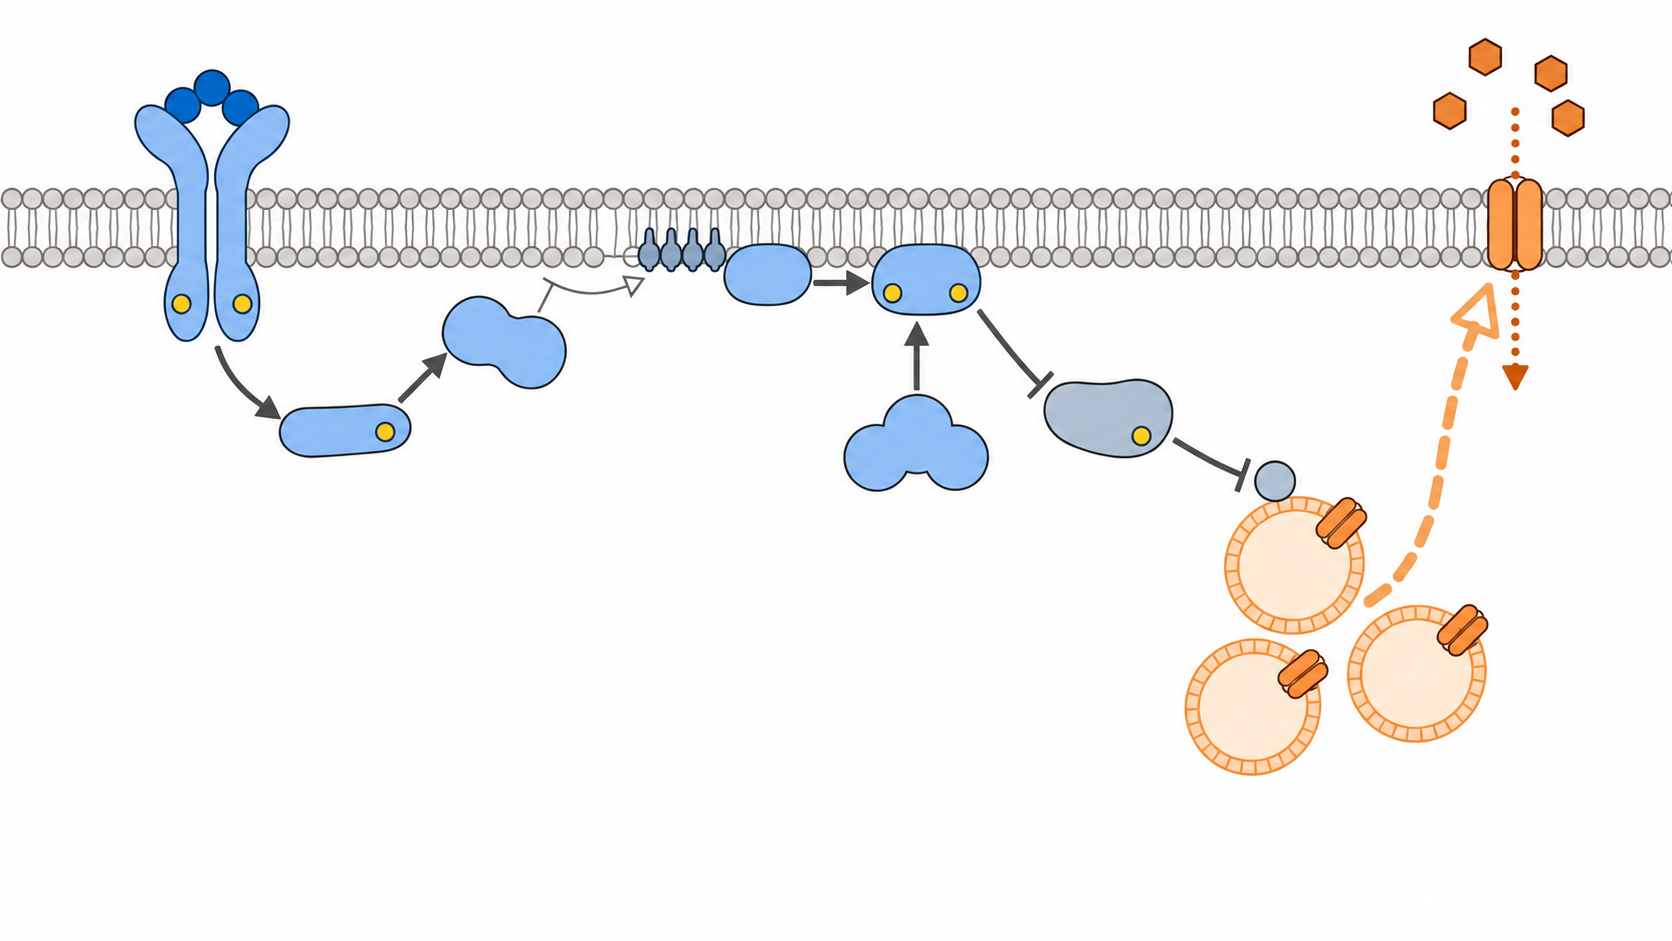
\includegraphics[width=\linewidth]{figures/ch07/ch07-06-v4-base.png}};
  \begin{scope}[x={(img.south east)}, y={(img.north west)},
    font=\sffamily\small]
    \node[text=ch07comp, font=\sffamily\footnotesize\itshape, anchor=west]
      at (0.04, 1-0.055) {胞外};
    \node[text=ch07comp, font=\sffamily\footnotesize\itshape]
      at (0.70, 1-0.15) {质膜};
    \node[text=ch07comp, font=\sffamily\footnotesize\itshape, anchor=west]
      at (0.04, 1-0.90) {胞质};
    \node[anchor=west, font=\sffamily\small] at (0.20, 1-0.06) {胰岛素};
    \draw[BookInk!40, thin] (0.20, 1-0.065) -- (0.145, 1-0.10);
    \node[anchor=west, font=\sffamily\small] at (0.20, 1-0.145) {胰岛素受体};
    \draw[BookInk!40, thin] (0.20, 1-0.15) -- (0.16, 1-0.20);
    \node[font=\sffamily\small] at (0.21, 1-0.56) {IRS-1};
    \node[font=\sffamily\small] at (0.34, 1-0.50) {PI3K};
    \node[font=\sffamily\footnotesize] at (0.47, 1-0.075) {PIP\textsubscript{2} → PIP\textsubscript{3}};
    \draw[BookInk!40, thin] (0.43, 1-0.10) -- (0.385, 1-0.275);
    \node[font=\sffamily\small] at (0.46, 1-0.40) {PDK1};
    \node[font=\sffamily\small] at (0.515, 1-0.375) {Akt};
    \draw[BookInk!40, thin] (0.53, 1-0.36) -- (0.55, 1-0.335);
    \node[font=\sffamily\small] at (0.52, 1-0.60) {mTORC2};
    \draw[BookInk!40, thin] (0.54, 1-0.56) -- (0.55, 1-0.52);
    \node[align=center, font=\sffamily\footnotesize] at (0.785, 1-0.345) {AS160\\（TBC1D4）};
    \draw[BookInk!40, thin] (0.745, 1-0.385) -- (0.695, 1-0.42);
    % Two short lines in the white gap right of the Rab circle (x 0.78–0.84).
    \node[align=left, font=\sffamily\scriptsize, anchor=south west] at (0.788, 1-0.508) {Rab-\\GTP};
    \draw[BookInk!40, thin] (0.784, 1-0.500) -- (0.770, 1-0.512);
    \node[font=\sffamily\small, anchor=north] at (0.78, 1-0.85) {GLUT4 储存囊泡};
    \draw[BookInk!40, thin] (0.78, 1-0.845) -- (0.78, 1-0.80);
    \node[font=\sffamily\small, anchor=west] at (0.94, 1-0.345) {GLUT4};
    \draw[BookInk!40, thin] (0.94, 1-0.33) -- (0.915, 1-0.26);
    \node[font=\sffamily\small, anchor=east] at (0.845, 1-0.065) {葡萄糖};
    \draw[BookInk!40, thin] (0.845, 1-0.075) -- (0.875, 1-0.09);
    % White gap beside the dashed arrow (the dashes sit near x=0.86).
    \node[text=ch07transnote, font=\sffamily\scriptsize\itshape, anchor=east]
      at (0.985, 1-0.455) {转位与融合};
    \draw[ch07transnote!55, thin] (0.876, 1-0.455) -- (0.858, 1-0.432);
  \end{scope}
  \node[anchor=north west, font=\sffamily\scriptsize, align=left] at (img.south west) {%
    \begin{tabular}{@{}l@{\quad}l@{}}
      \tikz{\draw[-{Stealth[length=1.5mm]}, ch07act, line width=0.6pt] (0,0) -- (0.22,0);} 激活 &
      \tikz{\draw[-{Bar[width=4pt]}, ch07act, line width=0.6pt] (0,0) -- (0.22,0);} 抑制 \\
      \tikz{\draw[ch07conv, line width=0.4pt] (0,0) .. controls (0.08,0.04) .. (0.18,0);} 酶促转化 &
      \tikz{\draw[ch07trans, line width=1pt, dashed] (0,0) -- (0.18,0);} 囊泡转位 \\
      \tikz{\draw[ch07flux, line width=0.6pt, dotted, -{Stealth[length=1.2mm]}] (0,0) -- (0.18,0);} 葡萄糖流动 &
      \tikz{\fill[ch07phos] (0.09,0) circle (1.2pt);} 磷酸化
    \end{tabular}};
\end{tikzpicture}

\caption{胰岛素刺激 GLUT4 转位的经典信号通路示意（终稿）。底图由图像模型生成且不含文字，标签与图例由 LaTeX 排版叠加。实线实心箭头表示激活，T 形端表示抑制，细弧线表示酶促转化，粗虚线表示囊泡转位，点线表示葡萄糖流动，琥珀色圆点表示磷酸化。图中省略了 MAPK 与 CAP–Cbl–TC10 分支、GLUT4 内吞与再循环、负反馈、SNARE 融合机器与细胞骨架运输，未区分 Akt 与 Rab 亚型，未画 mTORC2 的上游调控。依据 Saltiel 与 Kahn（2001）、Leto 与 Saltiel（2012）、Klip 等（2019）整理。完整图注见正文。}\label{fig:ch07-06}
\end{figure}

\subsection{完整图注、自查与核验记录}

若使用 SciDraw AI“图注辅助”（\sdtool{figure-legend}）起草图注，只能将其作为初稿，绝不能让工具补写样本量或统计检验。本案例的完整中英文图注如下：

\begin{BookNote}
\textbf{图 1　胰岛素刺激 GLUT4 转位的经典信号通路示意。} 胰岛素与质膜上的胰岛素受体结合，引起受体胞内段酪氨酸自身磷酸化，进而磷酸化 IRS-1 并招募 I A 类 PI3K。PI3K 在质膜内叶将 $\text{PIP}_2$ 转化为 $\text{PIP}_3$，后者招募 PDK1 与 Akt；Akt 由 PDK1 和 mTORC2 磷酸化而激活。活化的 Akt 磷酸化 AS160（TBC1D4），抑制其 Rab-GAP 活性，使 GLUT4 储存囊泡上的 Rab 维持 GTP 结合状态，促进囊泡向质膜转位并融合，GLUT4 由此增加于质膜，葡萄糖经其易化扩散进入细胞。实线实心箭头表示激活，T 形端表示抑制，细弧线表示酶促转化，粗虚线表示囊泡转位，点线表示葡萄糖流动，琥珀色圆点表示磷酸化。为便于阅读，图中省略了 MAPK 与 CAP–Cbl–TC10 分支、GLUT4 内吞与再循环、负反馈调节、SNARE 融合机器及细胞骨架运输；Rab 未区分具体亚型，Akt 未区分亚型，骨骼肌中并行的 TBC1D1 未画出；mTORC2 的上游激活方式未表示。依据 Saltiel 与 Kahn（2001）、Leto 与 Saltiel（2012）、Klip 等（2019）的综述整理。

\medskip
\textbf{Figure 1 | Schematic of the canonical insulin signaling pathway leading to GLUT4 translocation.} Insulin binding to the insulin receptor at the plasma membrane triggers tyrosine autophosphorylation of the receptor's intracellular domain, which phosphorylates IRS-1 and recruits class IA PI3K. PI3K converts $\text{PIP}_2$ to $\text{PIP}_3$ in the inner leaflet; $\text{PIP}_3$ recruits PDK1 and Akt, and Akt is activated by phosphorylation by PDK1 and mTORC2. Active Akt phosphorylates AS160 (TBC1D4), inhibiting its Rab-GAP activity. Rab proteins on GLUT4 storage vesicles therefore remain GTP-bound, promoting vesicle translocation to and fusion with the plasma membrane. The resulting increase in surface GLUT4 allows facilitated diffusion of glucose into the cell. Solid lines with filled heads, activation; T-bars, inhibition; thin arc, enzymatic conversion; thick dashed arrow, vesicle translocation; dotted arrow, glucose flux; amber dots, phosphorylation. For clarity, the MAPK and CAP–Cbl–TC10 branches, GLUT4 endocytosis and recycling, negative feedback, the SNARE fusion machinery and cytoskeletal transport are omitted; Rab and Akt isoforms are not distinguished, the parallel role of TBC1D1 in skeletal muscle is not shown, and upstream regulation of mTORC2 is not depicted. Based on reviews by Saltiel and Kahn (2001), Leto and Saltiel (2012) and Klip et al.\ (2019).
\end{BookNote}

逐句自查可见：前三句依次对应 R1–R4、R5–R8、R9–R13；第四句定义六项图例；第五句交代全部简化与省略；第六句写明文献依据，全段无任何数据或统计词。表~\ref{tab:ch07-verify} 展示了 V4 底图的实测核验记录：其中“核验人”与“领域同行复核人”必须分列，AI 与技术检查均不能替代同行复核。

\begin{table}[htbp]\centering\footnotesize
\setlength{\tabcolsep}{3pt}
\renewcommand{\arraystretch}{1.05}
\caption{GLUT4 主案例底图（V4）核验记录节选。核验人：第一作者；领域同行复核人：同领域合作者（待复核签字）。}\label{tab:ch07-verify}
\begin{tabularx}{\linewidth}{lYYYY}
\toprule
\textbf{检查项} & \textbf{任务书期望} & \textbf{V4 底图实测结果} & \textbf{结论} & \textbf{处置方式} \\
\midrule
R1–R4、R7–R8、R13 & 配体接触、磷酸化点、4 条激活线、mTORC2 无上游线、点线穿膜 & 对象计数、方向、圆点与线型均与任务书一致 & 通过 & 保持并叠加标签 \\
R5 酶促转化 & $\text{PIP}_2 \rightarrow \text{PIP}_3$ 细弧开放 V 头，PI3K 短线触中点 & 弧向右，但头为闭合空心三角，短线接在弧左端 & 部分偏差 & 教学稿记录在案；正式投稿可由 TikZ 重画 \\
R6 膜招募 & PDK1、Akt 紧贴内叶 $\text{PIP}_3$ 处，无箭头 & 均贴膜内叶且无箭头，但 Akt 距 $\text{PIP}_3$ 头基稍远 & 部分偏差 & 标签置于 PI3K 与 PDK1 之间辅助定位 \\
R9–R10 双重抑制 & Akt $\dashv$ AS160 $\dashv$ Rab 两条垂直 T 端紧贴靶标 & 串联 T 形线方向正确，Rab 贴左上囊泡，T 端留有窄白隙 & 部分偏差 & 语义清楚；严苛场景可改用方案 B 绘线 \\
R11–R12 转位融合 & 橙色粗虚线指向膜 GLUT4，囊泡 GLUT4 嵌膜 & 3 囊泡各嵌 1 个 GLUT4，粗虚线终点距膜 GLUT4 有小隙 & 部分偏差 & 虚线旁加“转位与融合”文字标签 \\
无字与分辨率 & 200\% 放大无文字；174 mm 通栏下达 300 ppi & 200\% 确认无文字；174 mm 宽下折算约 244 ppi & 待提分辨率 & 标为待修底图，不用插值冒充原生分辨率 \\
意外变化记录 & 记录修订中未要求的改动 & V3 无参考重生成丢磷酸化点并多出箭头；V4 无参考生成将囊泡 GLUT4 画入腔内 & 已拦截 & 改用上一版合格图作参考图后恢复正常 \\
\bottomrule
\end{tabularx}
\end{table}

\section{结构示意图：层序、材料与方向}

工程与材料领域的结构示意图（如电池截面、光伏叠层、催化膜组件），其核验对象从“逻辑关系”变成了四个物理维度：\textbf{层序}（哪层挨着哪层）、\textbf{材料对应}（哪种集流体配哪个电极）、\textbf{过程方向}（离子与电子各走哪条路）与\textbf{状态}（充电还是放电）。

假设一位做正极材料的硕士生要在论文引言中放一张锂离子软包电池单元截面图。她若只输入一句 \texttt{Draw a lithium-ion battery cross-section showing how it charges}，得到的图常在层序或离子方向上出错。依据电化学共识（Goodenough 与 Park，2013；Tarascon 与 Armand，2001；Armand 与 Tarascon，2008；电解液见 Xu，2004；隔膜见 Arora 与 Zhang，2004；材料见 Nitta 等，2015），我们先把核查标准列成表~\ref{tab:ch07-03}（S1–S8）。

\begin{table}[htbp]\centering\footnotesize
\caption{锂离子软包电池单元截面图的层序与过程核对表（S1–S8）。}\label{tab:ch07-03}
\begin{tabularx}{\linewidth}{lYYYY}
\toprule
\textbf{编号} & \textbf{项目} & \textbf{正确表述} & \textbf{常见错误} & \textbf{依据} \\
\midrule
S1 & 层序（自左至右） & 外壳铝塑膜 $\rightarrow$ 铜集流体 $\rightarrow$ 负极（石墨）涂层 $\rightarrow$ 隔膜 $\rightarrow$ 正极（如 $\text{LiCoO}_2$）涂层 $\rightarrow$ 铝集流体 $\rightarrow$ 外壳铝塑膜 & 隔膜放在电极与集流体之间、两电极直接接触 & Goodenough 与 Park，2013；Arora 与 Zhang，2004 \\
S2 & 集流体与电极对应 & 负极用铜箔，正极用铝箔 & 两者对调 & Nitta 等，2015；行业与教科书约定 \\
S3 & 电解液位置 & 浸润两电极孔隙和隔膜孔隙 & 只画成两极之间的一条独立“液体层” & Xu，2004 \\
S4 & 充电时 $\text{Li}^+$ & 由正极脱出，经电解液/隔膜迁移，嵌入石墨负极（右 $\rightarrow$ 左） & 方向画反（左 $\rightarrow$ 右） & Goodenough 与 Park，2013 \\
S5 & 充电时电子 & 由正极经外电路（充电器）流向负极 & 电子穿过隔膜/电解液 & 同上 \\
S6 & 放电时 $\text{Li}^+$ / 电子 & $\text{Li}^+$ 负极 $\rightarrow$ 正极（左 $\rightarrow$ 右）经电解液；电子负极 $\rightarrow$ 外电路（负载）$\rightarrow$ 正极 & 方向未随状态反转 & 同上 \\
S7 & $\text{Li}^+$ 路径 & 只在电池内部（电解液）中迁移 & $\text{Li}^+$ 被画进外电路导线 & 同上 \\
S8 & 命名 & 图中写“负极/正极”；必要时在图注说明 anode/cathode 按放电约定命名 & 充电图中写 anode/cathode 而不说明，或两者对调 & 教科书约定 \\
\bottomrule
\end{tabularx}
\end{table}

我们先按设计的错误提示词生成图~\ref{fig:ch07-07}，供读者对照表~\ref{tab:ch07-03} 找错：（1）左侧石墨负极画了银灰铝箔、右侧正极画了铜色铜箔（集流体与电极配对颠倒，违反 S2）；（2）石墨片层与灰蓝球形正极颗粒直接挨在一起（实际电池中意味着内短路），白色多孔隔膜被错放到正极与右侧铜箔之间（层序错误，违反 S1）；（3）顶部标为“充电”，但电极内六个橙色 $\text{Li}^+$ 圆球全部向右移动，即从负极流向正极（充电迁移方向画反，违反 S4）；（4）顶部外电路导线上也画了三个带箭头的橙色 $\text{Li}^+$ 圆球（离子误入外电路，违反 S7）。

\begin{figure}[htbp]\centering
% FIG ch07-07 battery common errors overlay (Chinese)
\definecolor{ch07err}{HTML}{C0392B}
\definecolor{ch07Li}{HTML}{D9822B}
\definecolor{ch07wire}{HTML}{3A3A3A}
\begin{tikzpicture}
  \node[anchor=south west, inner sep=0] (img) at (0,0)
    {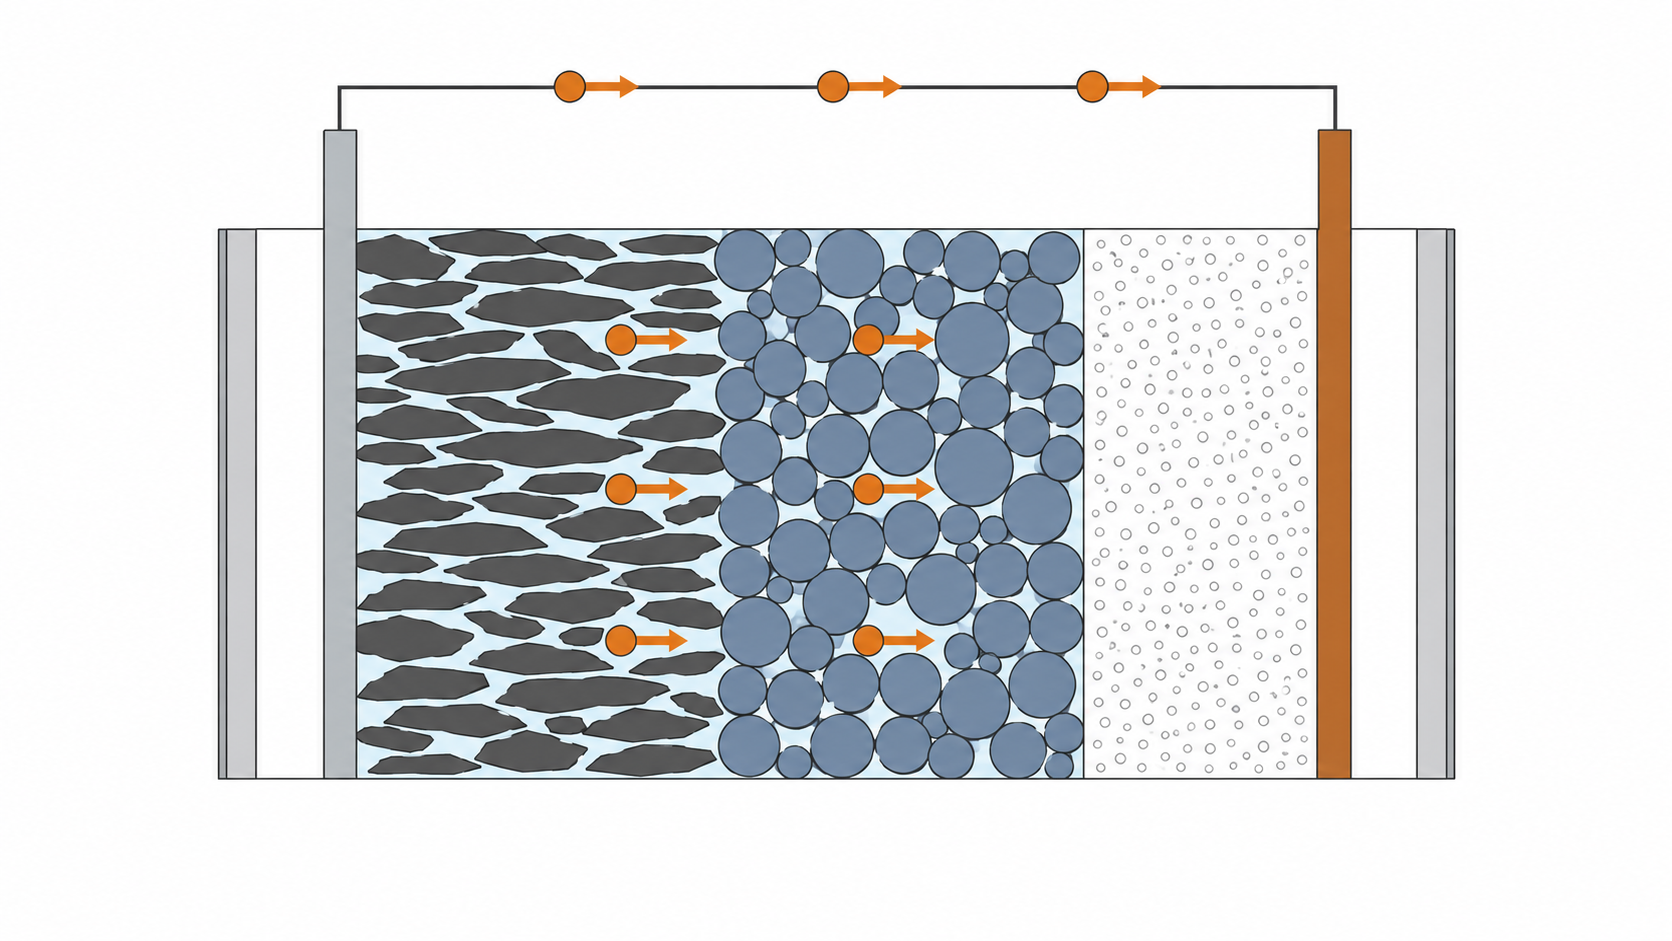
\includegraphics[width=\linewidth]{figures/ch07/ch07-07-battery-errors.png}};
  \begin{scope}[x={(img.south east)}, y={(img.north west)},
    font=\sffamily\small]
    \node[font=\bfseries] at (0.50, 1-0.02) {充电（错误示例）};
    \node[font=\scriptsize] at (0.20, 1-0.90) {铝箔};
    \node[font=\scriptsize, align=center] at (0.315, 1-0.90) {负极\\（石墨）};
    \node[font=\scriptsize, align=center] at (0.525, 1-0.90) {正极\\（如 LiCoO$_2$）};
    \node[font=\scriptsize] at (0.69, 1-0.90) {隔膜};
    \node[font=\scriptsize] at (0.76, 1-0.94) {铜箔};
    \node[font=\scriptsize, rotate=90, anchor=south] at (0.15, 1-0.20) {外壳};
    \node[font=\scriptsize] at (0.20, 1-0.11) {负极极耳};
    \node[font=\scriptsize] at (0.76, 1-0.11) {正极极耳};
    \node[font=\scriptsize\bfseries, text=white, fill=ch07err, circle, inner sep=1.5pt] at (0.20, 1-0.22) {❶};
    \node[font=\scriptsize\bfseries, text=white, fill=ch07err, circle, inner sep=1.5pt] at (0.76, 1-0.22) {❶};
    \node[font=\scriptsize\bfseries, text=white, fill=ch07err, circle, inner sep=1.5pt] at (0.42, 1-0.22) {❷};
    \node[font=\scriptsize\bfseries, text=white, fill=ch07err, circle, inner sep=1.5pt] at (0.40, 1-0.55) {❸};
    \node[font=\scriptsize\bfseries, text=white, fill=ch07err, circle, inner sep=1.5pt] at (0.50, 1-0.08) {❹};
    \node[font=\scriptsize, text=BookInk!80, anchor=north] at (0.50, 1-0.96)
      {❶–❹ 对应表~7-3 的 S2、S1、S4、S7};
  \end{scope}
\end{tikzpicture}

\caption{一张有意构造的错误电池结构示意（图像模型按“错误”要求生成）。❶ 铜、铝集流体对调；❷ 隔膜不在两电极之间，两极直接接触（实际电池中意味着内短路）；❸ 标为充电，但 $\text{Li}^+$ 从负极流向正极；❹ $\text{Li}^+$ 被画进外电路。对照正确画法见图~\ref{fig:ch07-08}。}\label{fig:ch07-07}
\end{figure}

为什么正确画法（图~\ref{fig:ch07-08}）不让图像模型画箭头？因为箭头方向是本图的核心科学内容，在充电与放电两种状态下恰好相反；若分两次生成，层厚与颗粒排布会发生随机漂移，读者会误以为充放电改变了宏观层结构。因此我们采用“结构底图只画一次，两套过程箭头全部在 TikZ 中叠加”的方案。任务书如下：

\begin{Prompt}
【用途与读者】论文引言/组会用结构示意图，单栏宽约 85 mm 两面板竖排，或双栏 174 mm 两面板并排；
读者为材料与化学方向的同行与研究生。
【目标】让读者看清一个锂离子电池单元的层序与材料对应，并区分充电与放电时 Li+ 和电子各自的路径与方向。
【材料】教科书级共识（Goodenough & Park 2013 等）；不含实验数据。
【对象】外壳铝塑膜（两侧）、铜集流体与负极极耳、石墨负极涂层、多孔隔膜、
正极涂层（层状氧化物，如 LiCoO2）、铝集流体与正极极耳、电解液（浸润孔隙）。每层只出现一次。
【关系/过程】结构底图中不画任何过程。叠加层：
(a) 充电：Li+ 正极 → 隔膜 → 负极；电子 正极极耳 → 充电器 → 负极极耳。
(b) 放电：Li+ 负极 → 隔膜 → 正极；电子 负极极耳 → 负载 → 正极极耳。
Li+ 只在电池内部；电子只在外电路。
【布局】横向截面，各层为竖直条带自左至右排列；极耳从集流体顶端伸出；
顶部留白给外电路，底部留白给图例。
【视觉】白底扁平二维；铜色、银灰、炭黑、灰蓝四种材料色加极浅蓝电解液；无渐变阴影 3D。
【限制】底图无任何文字、符号、离子、箭头、导线；不画 SEI、黏结剂、导电剂、分子结构；厚度不按比例。
【图例】Li+ 迁移（橙色实线实心头）、电子流（深灰虚线）、电解液（浅蓝）。
【验收】S1–S8 全部正确；两面板底图为同一文件；图注说明简化与命名约定。
\end{Prompt}

按上述任务书生成结构底图时，我们将同一提示词生成了三次：第一次在外壳膜与集流体之间多画了两条浅蓝竖带，看起来像独立的液体层（违反 S3）；第三次隔膜圆孔发白且正极颗粒过稀；第二次生成的结果严格呈现“外壳膜—铜集流体—片状石墨负极—中央多孔隔膜—球形正极—铝集流体—外壳膜”的层序，且无任何离子、导线或文字（放大检查仅见隔膜个别孔隙的浅蓝填充略有不均）。排版时，我们把这一张底图并排调用两次，在 TikZ 中分别叠加上方外电路（充电器或负载）、电子流虚线（$\text{e}^-$）与内部穿过隔膜的 $\text{Li}^+$ 橙色实线箭头（图~\ref{fig:ch07-08}）。顺带说明：把位图转成 PPTX 或 SVG 只能分离文字与背景，不会把颗粒或隔膜变成带科研语义的矢量对象，因此方向箭头仍应在 TikZ 或排版软件中绘制。

\begin{figure}[htbp]\centering
% FIG ch07-08 charge/discharge overlay (Chinese) — shared structural base, twice
\definecolor{ch07Li}{HTML}{D9822B}
\definecolor{ch07wire}{HTML}{3A3A3A}
\definecolor{ch07elec}{HTML}{3A3A3A}
\definecolor{ch07electrolyte}{HTML}{E3F0F8}
\makeatletter
\@ifundefined{chsevenpanelbase}{%
  \newcommand{\chsevenpanelbase}{figures/ch07/ch07-08-battery-base.png}
}{}
\@ifundefined{chsevendrawcircuit}{%
\newcommand{\chsevendrawcircuit}[1]{%
  \def\ChSevenWireY{1.10}%
  \def\ChSevenTabY{0.878}%
  \draw[ch07wire, line width=0.8pt] (0.194, \ChSevenTabY) -- (0.194, \ChSevenWireY);
  \draw[ch07wire, line width=0.8pt] (0.805, \ChSevenTabY) -- (0.805, \ChSevenWireY);
  \draw[ch07wire, line width=0.8pt] (0.194, \ChSevenWireY) -- (0.805, \ChSevenWireY);
  \node[draw=ch07wire, line width=0.6pt, rounded corners=1.5pt, fill=white,
    font=\sffamily\scriptsize, inner sep=1.6pt]
    at (0.50, \ChSevenWireY) {#1};
  \foreach \chyy in {0.38, 0.52, 0.66} {%
    \draw[-{Stealth[length=2mm]}, ch07Li, line width=0.9pt]
      (0.68, 1-\chyy) -- (0.32, 1-\chyy);
  }%
  \node[font=\sffamily\scriptsize, text=ch07Li, fill=white, inner sep=0.7pt]
    at (0.50, 1-0.30) {Li\textsuperscript{+}};
  \draw[ch07elec, line width=0.7pt, dashed, -{Stealth[length=1.5mm]}]
    (0.76, \ChSevenWireY) -- (0.62, \ChSevenWireY);
  \draw[ch07elec, line width=0.7pt, dashed, -{Stealth[length=1.5mm]}]
    (0.38, \ChSevenWireY) -- (0.24, \ChSevenWireY);
}
}{}
\@ifundefined{chsevendrawcircuitb}{%
\newcommand{\chsevendrawcircuitb}[1]{%
  \def\ChSevenWireY{1.10}%
  \def\ChSevenTabY{0.878}%
  \draw[ch07wire, line width=0.8pt] (0.194, \ChSevenTabY) -- (0.194, \ChSevenWireY);
  \draw[ch07wire, line width=0.8pt] (0.805, \ChSevenTabY) -- (0.805, \ChSevenWireY);
  \draw[ch07wire, line width=0.8pt] (0.194, \ChSevenWireY) -- (0.805, \ChSevenWireY);
  \node[draw=ch07wire, line width=0.6pt, rounded corners=1.5pt, fill=white,
    font=\sffamily\scriptsize, inner sep=1.6pt]
    at (0.50, \ChSevenWireY) {#1};
  \foreach \chyy in {0.38, 0.52, 0.66} {%
    \draw[-{Stealth[length=2mm]}, ch07Li, line width=0.9pt]
      (0.32, 1-\chyy) -- (0.68, 1-\chyy);
  }%
  \node[font=\sffamily\scriptsize, text=ch07Li, fill=white, inner sep=0.7pt]
    at (0.50, 1-0.30) {Li\textsuperscript{+}};
  \draw[ch07elec, line width=0.7pt, dashed, -{Stealth[length=1.5mm]}]
    (0.24, \ChSevenWireY) -- (0.38, \ChSevenWireY);
  \draw[ch07elec, line width=0.7pt, dashed, -{Stealth[length=1.5mm]}]
    (0.62, \ChSevenWireY) -- (0.76, \ChSevenWireY);
}
}{}
\makeatother
\begin{tikzpicture}
  \node[anchor=south west, inner sep=0] (imgA) at (0,0)
    {\includegraphics[width=0.49\linewidth]{\chsevenpanelbase}};
  \node[anchor=south west, inner sep=0] (imgB) at (0.51\linewidth,0)
    {\includegraphics[width=0.49\linewidth]{\chsevenpanelbase}};
  \begin{scope}[shift={(imgA.south west)},
    x={($(imgA.south east)-(imgA.south west)$)},
    y={($(imgA.north west)-(imgA.south west)$)},
    font=\sffamily\small]
    \node[anchor=south west, font=\sffamily\small] at (0.00, 1.20) {\textbf{(a)} 充电};
    \node[font=\sffamily\scriptsize, anchor=north west] at (0.25, 1.045) {负极极耳};
    \node[font=\sffamily\scriptsize, anchor=north east] at (0.75, 1.045) {正极极耳};
    \chsevendrawcircuit{充电器}
  \end{scope}
  \begin{scope}[shift={(imgB.south west)},
    x={($(imgB.south east)-(imgB.south west)$)},
    y={($(imgB.north west)-(imgB.south west)$)},
    font=\sffamily\small]
    \node[anchor=south west, font=\sffamily\small] at (0.00, 1.20) {\textbf{(b)} 放电};
    \chsevendrawcircuitb{负载}
  \end{scope}
  \begin{scope}[shift={(imgA.south west)},
    x={($(imgA.south east)-(imgA.south west)$)},
    y={($(imgA.north west)-(imgA.south west)$)},
    font=\sffamily\scriptsize]
    \node[align=center, anchor=north] at (0.323, 0.19) {负极\\（石墨）};
    \node[anchor=north] at (0.50, 0.19) {隔膜};
    \node[align=center, anchor=north] at (0.678, 0.19) {正极\\（LiCoO\textsubscript{2}）};
    \draw[BookInk!45, thin] (0.193, 0.19) -- (0.193, -0.02);
    \node[align=center, anchor=north] at (0.193, -0.02) {铜\\集流体};
    \draw[BookInk!45, thin] (0.806, 0.19) -- (0.806, -0.02);
    \node[align=center, anchor=north] at (0.806, -0.02) {铝\\集流体};
  \end{scope}
  \node[anchor=north, font=\sffamily\scriptsize, align=center] at (0.5\linewidth, -0.13\linewidth) {%
    \begin{tabular}{@{}c@{\qquad}c@{}}
      \tikz{\draw[-{Stealth[length=1.5mm]}, ch07Li, line width=0.7pt] (0,0) -- (0.2,0);} Li\textsuperscript{+} 迁移（电解液中） &
      \tikz{\draw[ch07elec, line width=0.6pt, dashed, -{Stealth[length=1.2mm]}] (0,0) -- (0.2,0);} 电子流（外电路） \\[0.4em]
      \multicolumn{2}{c}{\tikz{\fill[ch07electrolyte] (0,0) rectangle (0.08,0.06);} 电解液（填充孔隙）} \\[0.35em]
      \multicolumn{2}{c}{两侧浅灰竖条为外壳}
    \end{tabular}};
\end{tikzpicture}

\caption{锂离子软包电池一个重复单元的截面示意。两面板使用同一张结构底图（图像模型生成，不含文字和箭头），箭头、外电路与标签由 LaTeX 叠加。（a）充电：$\text{Li}^+$ 从正极脱出，经电解液穿过隔膜嵌入石墨负极，电子经外电路由正极流向负极。（b）放电：方向相反，电子经负载由负极流向正极。负极使用铜集流体，正极使用铝集流体；电解液浸润电极与隔膜的孔隙。各层厚度不按比例（隔膜被加宽），只画一个单元（实际软包由多层双面涂布极片叠片或卷绕），省略 SEI、黏结剂、导电剂与封装细节；“负极/正极”即按放电约定所称的阳极/阴极。}\label{fig:ch07-08}
\end{figure}

\section{AI 能做什么、不能做什么、作者要核对什么}

表~\ref{tab:ch07-02} 汇总了机制图与结构示意图各环节中 AI（含 SciDraw AI）的能力边界与作者必须核对的事项。

\begin{table}[htbp]\centering\footnotesize
\caption{机制图与结构示意图制作中 AI 能做、不能做与作者核对事项对照表。}\label{tab:ch07-02}
\begin{tabularx}{\linewidth}{lYYY}
\toprule
\textbf{环节} & \textbf{AI（含 SciDraw AI）能做} & \textbf{AI 不能做} & \textbf{作者要核对} \\
\midrule
整理关系 & 把作者写好的关系表改写成提示词段落；在科研绘图向导中按“机制图与流程图”路线组织任务书 & 判断某条关系是否已确立、是否有争议；自动阅读整篇论文并找出正确机制 & 每条关系都有文献依据；确立 / 简化 / 假设的标注；“不画的内容”清单 \\
草图与布局 & 草图模式把草图与文字一起作为生成输入，给出大致遵循布局的候选图 & 保证布局硬性保持或对象锁定；同一提示词两次给出相同排布 & 分区、阅读路径、对象数量；与草图的偏差 \\
生成底图 & 机制图生成或提示词绘图按任务书产出扁平风格的无字候选图；批量候选 & 保证不多画、不漏画、不出现伪文字；保证色值和线宽精确 & 用核验表逐条核对 R1–R13 或 S1–S8；放大检查伪字符 \\
修改 & 选择历史图并输入修改指令，进行连续迭代 & 只改指定之处而不影响其他部分 & 每次修改后全表复核，记录意外变化 \\
线型与颜色 & 按提示词中定义的线型与色板绘制；图片检查给出灰度、色觉风险、分辨率等技术报告 & 自行决定线型的科学含义；技术检查不代表科学审核 & 图例与线型一一对应；颜色只承担角色；灰度可辨 \\
标签与方向 & 无（本章做法：标签与关键箭头不交给图像模型） & 可靠拼写分子名、上下标；在不同状态下保持结构不变而只翻转方向 & 标签逐字从清单复制；箭头方向与过程状态一致 \\
图注 & 图注辅助根据图片起草图注草稿 & 知道作者省略了什么、依据哪篇文献；补写样本量或统计（本类图本就不应出现） & 每句对应关系表；简化与省略写全；中英文各自通顺 \\
交付 & 组图工具排版与导出（第九章） & 图像转 PPTX/SVG 不会把底图变成带科研语义的可编辑对象 & 终稿文字为排版文字；底图分辨率足够；同行复核 \\
\bottomrule
\end{tabularx}
\end{table}

\section{本章检查清单}

\begin{itemize}
\item 先有关系表（起点、终点、关系类型、位置、证据状态），再写提示词；列出“不画的内容”。
\item 每个对象出现次数明确；允许重复的对象（如 GLUT4 的储存态与膜上态）在任务书中写明。
\item 空间分区（胞外/膜/胞质，或结构图的层序）写进任务书，并在图中可辨。
\item 每种关系类型只用一种线型；图例定义全部线型；假设关系与确立关系可区分。
\item 没有“捷径箭头”：间接作用（如“抑制的抑制”）保留中间环节。
\item 颜色只编码角色，色相不超过 3 个加灰色；灰度下关系仍可读。
\item 底图放大检查无伪文字、无多余对象；所有标签由排版生成，逐字从清单复制。
\item 结构图：层序、材料对应、过程方向、状态（如充电/放电）逐项核对；结构只画一次，状态用叠加层区分。
\item 每次 AI 修改后完整复核，而不只看改动处；记录意外变化。
\item 图注写明简化、省略与依据；不写任何数据或统计。
\item 至少一位领域同行复核关系与结构。
\end{itemize}

\section{本章练习}

\begin{enumerate}
\item \textbf{拆捷径箭头（纸笔）。} 常见教学图写着“$\text{Akt} \rightarrow \text{GLUT4 translocation}$”。（a）写出省略的中间环节，并为每一环指定图~\ref{fig:ch07-01} 中的线型；（b）解释为什么 Akt 与 AS160 之间画抑制线，而整条通路的净效应是促进转位；（c）写成三行关系表（起点、终点、关系、线型、依据），注明你查阅的综述及其具体部分。

\item \textbf{SciDraw AI 实操：同一机制，两种输入。} 选一条你领域中教科书已确立、不超过 8 个对象的机制。（a）在科研绘图向导选择“机制图与流程图”路线，按十个填写项写任务书（必须含空间分区与线型定义），下载副本；（b）先在机制图生成中只输入一句话，按本章核验表记录至少 5 处问题；（c）再粘贴完整任务书生成无字底图，比较两份核验表；（d）选一张历史图输入一条修改指令，记录至少一处“意外变化”。提交两张图、两份核验表、一条修改指令和修改记录。

\item \textbf{结构图找错与改正。} 以质子交换膜燃料电池（PEMFC）单电池截面为对象（或你领域的另一种层状器件）：（a）写出自左至右的层序与每层材料，以及工作时 $\text{H}^+$、电子、$\text{H}_2/\text{O}_2/\text{H}_2\text{O}$ 各自的路径和方向，并给出依据文献；（b）设计一张故意含 3 处错误的提示词，再写一份正确的结构底图提示词（不含箭头与文字）；（c）用 TikZ 在正确底图上叠加过程箭头与标签，并用灰度打印检查线型可辨。
\end{enumerate}

\section*{参考文献}

\begin{itemize}
\item Armand M, Tarascon JM. Building better batteries. \emph{Nature}. 2008;451(7179):652--657. doi:10.1038/451652a
\item Arora P, Zhang Z. Battery separators. \emph{Chem Rev}. 2004;104(10):4419--4462. doi:10.1021/cr020738u
\item ColorBrewer 2.0: Color advice for cartography and scientific visualization. \url{https://colorbrewer2.org/}
\item Goodenough JB, Park KS. The Li-ion rechargeable battery: a perspective. \emph{J Am Chem Soc}. 2013;135(4):1167--1176. doi:10.1021/ja3091438
\item Klip A, McGraw TE, James DE. Thirty sweet years of GLUT4. \emph{J Biol Chem}. 2019;294(30):11369--11381. doi:10.1074/jbc.REV119.008351
\item Le Nov\`ere N, Hucka M, Mi H, Moodie S, Schreiber F, Sorokin A, et al. The Systems Biology Graphical Notation. \emph{Nat Biotechnol}. 2009;27(8):735--741. doi:10.1038/nbt.1558
\item Leto D, Saltiel AR. Regulation of glucose transport by insulin: traffic control of GLUT4. \emph{Nat Rev Mol Cell Biol}. 2012;13(6):383--396. doi:10.1038/nrm3351
\item Nitta N, Wu F, Lee JT, Yushin G. Li-ion battery materials: present and future. \emph{Mater Today}. 2015;18(5):252--264. \path{doi:10.1016/j.mattod.2014.10.040}
\item Rougier NP, Droettboom M, Bourne PE. Ten simple rules for better figures. \emph{PLoS Comput Biol}. 2014;10(9):e1003833. \path{doi:10.1371/journal.pcbi.1003833}
\item Saltiel AR, Kahn CR. Insulin signalling and the regulation of glucose and lipid metabolism. \emph{Nature}. 2001;414(6865):799--806. doi:10.1038/414799a
\item Sano H, Kane S, Sano E, M\^{\i}inea CP, Asara JM, Lane WS, Garner CW, Lienhard GE. Insulin-stimulated phosphorylation of a Rab GTPase-activating protein regulates GLUT4 translocation. \emph{J Biol Chem}. 2003;278(17):14599--14602. doi:10.1074/jbc.C300063200
\item Sarbassov DD, Guertin DA, Ali SM, Sabatini DM. Phosphorylation and regulation of Akt/PKB by the Rictor-mTOR complex. \emph{Science}. 2005;307(5712):1098--1101. doi:10.1126/science.1106148
\item Systems Biology Graphical Notation (SBGN) official website. \url{https://sbgn.github.io/}
\item Tarascon JM, Armand M. Issues and challenges facing rechargeable lithium batteries. \emph{Nature}. 2001;414(6861):359--367. doi:10.1038/35104644
\item Wong B. Points of view: Color blindness. \emph{Nat Methods}. 2011;8(6):441. doi:10.1038/nmeth.1618
\item Xu K. Nonaqueous liquid electrolytes for lithium-based rechargeable batteries. \emph{Chem Rev}. 2004;104(10):4303--4418. doi:10.1021/cr030203g
\end{itemize}
